%%%%%%%%%%%%%%%%%%%%%%%%%%%%%%%%%%%%%%%%%
% Masters/Doctoral Thesis 
% LaTeX Template
% Version 2.5 (27/8/17)
%
% This template was downloaded from:
% http://www.LaTeXTemplates.com
%
% Version 2.x major modifications by:
% Vel (vel@latextemplates.com)
%
% This template is based on a template by:
% Steve Gunn (http://users.ecs.soton.ac.uk/srg/softwaretools/document/templates/)
% Sunil Patel (http://www.sunilpatel.co.uk/thesis-template/)
%
% Template license:
% CC BY-NC-SA 3.0 (http://creativecommons.org/licenses/by-nc-sa/3.0/)
%
%%%%%%%%%%%%%%%%%%%%%%%%%%%%%%%%%%%%%%%%%



%----------------------------------------------------------------------------------------
%	PACKAGES AND OTHER DOCUMENT CONFIGURATIONS
%----------------------------------------------------------------------------------------

\documentclass[
11pt, % The default document font size, options: 10pt, 11pt, 12pt
%oneside, % Two side (alternating margins) for binding by default, uncomment to switch to one side
english, % ngerman for German
singlespacing, % Single line spacing, alternatives: onehalfspacing or doublespacing
% draft, % Uncomment to enable draft mode (no pictures, no links, overfull hboxes indicated)
%nolistspacing, % If the document is onehalfspacing or doublespacing, uncomment this to set spacing in lists to single
%liststotoc, % Uncomment to add the list of figures/tables/etc to the table of contents
%toctotoc, % Uncomment to add the main table of contents to the table of contents
parskip, % Uncomment to add space between paragraphs
%nohyperref, % Uncomment to not load the hyperref package
headsepline, % Uncomment to get a line under the header
%chapterinoneline, % Uncomment to place the chapter title next to the number on one line
%consistentlayout, % Uncomment to change the layout of the declaration, abstract and acknowledgements pages to match the default layout
dvipsnames]{misc/MastersDoctoralThesis} % The class file specifying the document structure


\usepackage[utf8]{inputenc} % Required for inputting international characters
\usepackage[T1]{fontenc} % Output font encoding for international characters
\usepackage{hyperref}
\usepackage{mathpazo} % Use the Palatino font by default

\usepackage[backend=biber,style=ieee]{biblatex} % Use the bibtex backend with the authoryear citation style (which resembles APA)

\addbibresource{references.bib} % The filename of the bibliography

\usepackage[autostyle=true]{csquotes} % Required to generate language-dependent quotes in the bibliography
\usepackage{float} % Improved interface for floating objects
\usepackage{booktabs}
\usepackage{pseudocode} % Environment for specifying algorithms in a natural way
\usepackage{multirow}
\usepackage{enumitem}% http://ctan.org/pkg/enumitem
\usepackage{amsthm, amsmath, amssymb} % Mathematical typesetting
\theoremstyle{definition}
\newtheorem{definition}{Definition}[section]
\usepackage{xcolor}
\newcommand\todo[1]{\textcolor{red}{#1}}
\usepackage{algorithm, algpseudocode}
\algnewcommand\algorithmicforeach{\textbf{for each}}
\algdef{S}[FOR]{ForEach}[1]{\algorithmicforeach\ #1\ \algorithmicdo}

\usepackage{nicematrix}
\NiceMatrixOptions{
code-for-first-row =\color{BurntOrange},
code-for-last-col =\color{RoyalBlue}
}
\setcounter{MaxMatrixCols}{8}
\allowdisplaybreaks
\setlength\doublerulesep{0.6pt}

%----------------------------------------------------------------------------------------
%	MARGIN SETTINGS
%----------------------------------------------------------------------------------------
\setlength{\parskip}{9pt}

\geometry{
	paper=a4paper, % Change to letterpaper for US letter
	inner=2.5cm, % Inner margin
	outer=3.8cm, % Outer margin
	bindingoffset=.5cm, % Binding offset
	top=1.5cm, % Top margin
	bottom=1.5cm, % Bottom margin
	% showframe, % Uncomment to show how the type block is set on the page
}

%----------------------------------------------------------------------------------------
%	THESIS INFORMATION
%----------------------------------------------------------------------------------------

\thesistitle{Cost Estimation for Factorized Machine Learning} % Your thesis title, this is used in the title and abstract, print it elsewhere with \ttitle
\supervisor{Dr. Rihan \textsc{Hai}} % Your supervisor's name, this is used in the title page, print it elsewhere with \supname
\examiner{} % Your examiner's name, this is not currently used anywhere in the template, print it elsewhere with \examname
\degree{Master of Science} % Your degree name, this is used in the title page and abstract, print it elsewhere with \degreename
\author{Pepijn te \textsc{Marvelde}} % Your name, this is used in the title page and abstract, print it elsewhere with \authorname
\addresses{} % Your address, this is not currently used anywhere in the template, print it elsewhere with \addressname

\subject{Computer Science} % Your subject area, this is not currently used anywhere in the template, print it elsewhere with \subjectname
\keywords{} % Keywords for your thesis, this is not currently used anywhere in the template, print it elsewhere with \keywordnames
\university{\href{http://www.tudelft.nl}{Delft University of Technology}} % Your university's name and URL, this is used in the title page and abstract, print it elsewhere with \univname
\department{\href{https://www.tudelft.nl/en/eemcs/the-faculty/departments/software-technology/}{Software Technology}} % Your department's name and URL, this is used in the title page and abstract, print it elsewhere with \deptname
\group{\href{http://www.wis.ewi.tudelft.nl/}{Web Information Systems Group}} % Your research group's name and URL, this is used in the title page, print it elsewhere with \groupname
\faculty{\href{https://www.tudelft.nl/en/ewi/}{Electrical Engineering, Mathematics and Computer Science}} % Your faculty's name and URL, this is used in the title page and abstract, print it elsewhere with \facname

\AtBeginDocument{
\hypersetup{pdftitle=\ttitle} % Set the PDF's title to your title
\hypersetup{pdfauthor=\authorname} % Set the PDF's author to your name
\hypersetup{pdfkeywords=\keywordnames} % Set the PDF's keywords to your keywords
}

\begin{document}

\frontmatter % Use roman page numbering style (i, ii, iii, iv...) for the pre-content pages

\pagestyle{plain} % Default to the plain heading style until the thesis style is called for the body content

%----------------------------------------------------------------------------------------
%	TITLE PAGE
%----------------------------------------------------------------------------------------

\begin{titlepage}
	\begin{center}

		\vspace*{.06\textheight}
		{\scshape\LARGE \univname\par}\vspace{1.5cm} % University name
		\textsc{\Large Master’s Thesis}\\[0.5cm] % Thesis type

		\HRule \\[0.4cm] % Horizontal line
		{\huge \bfseries \ttitle\par}\vspace{0.4cm} % Thesis title
		\HRule \\[1.5cm] % Horizontal line

		\begin{minipage}[t]{0.4\textwidth}
			\begin{flushleft} \large
				\emph{Author:}\\
				\href{http://www.johnsmith.com}{\authorname} % Author name - remove the \href bracket to remove the link
			\end{flushleft}
		\end{minipage}
		\begin{minipage}[t]{0.4\textwidth}
			\begin{flushright} \large
				\emph{Supervisor:} \\
				\href{http://www.jamessmith.com}{\supname} % Supervisor name - remove the \href bracket to remove the link  
			\end{flushright}
		\end{minipage}\\[3cm]

		\vfill

		\large \textit{A thesis submitted in fulfillment of the requirements\\ for the degree of \degreename}\\[0.3cm] % University requirement text
		\textit{in the}\\[0.4cm]
		\groupname\\\deptname\\[2cm] % Research group name and department name

		\vfill

		{\large \today}\\[4cm] % Date
		%\includegraphics{Logo} % University/department logo - uncomment to place it

		\vfill
	\end{center}
\end{titlepage}

%----------------------------------------------------------------------------------------
%	DECLARATION PAGE
%----------------------------------------------------------------------------------------

\begin{declaration}
	\addchaptertocentry{\authorshipname} % Add the declaration to the table of contents
	\noindent I, \authorname, declare that this thesis titled, \enquote{\ttitle} and the work presented in it are my own. I confirm that:

	\begin{itemize}
		\item This work was done wholly or mainly while in candidature for a research degree at this University.
		\item Where any part of this thesis has previously been submitted for a degree or any other qualification at this University or any other institution, this has been clearly stated.
		\item Where I have consulted the published work of others, this is always clearly attributed.
		\item Where I have quoted from the work of others, the source is always given. With the exception of such quotations, this thesis is entirely my own work.
		\item I have acknowledged all main sources of help.
		\item Where the thesis is based on work done by myself jointly with others, I have made clear exactly what was done by others and what I have contributed myself.\\
	\end{itemize}

	\noindent Signed:\\
	\rule[0.5em]{25em}{0.5pt} % This prints a line for the signature

	\noindent Date:\\
	\rule[0.5em]{25em}{0.5pt} % This prints a line to write the date
\end{declaration}

\cleardoublepage

%----------------------------------------------------------------------------------------
%	QUOTATION PAGE
%----------------------------------------------------------------------------------------

% \vspace*{0.2\textheight}

% \noindent\enquote{\itshape Thanks to my solid academic training, today I can write hundreds of words on virtually any topic without possessing a shred of information, which is how I got a good job in journalism.}\bigbreak

% \hfill Dave Barry

%----------------------------------------------------------------------------------------
%	ABSTRACT PAGE
%----------------------------------------------------------------------------------------

\begin{abstract}
	\addchaptertocentry{\abstractname} % Add the abstract to the table of contents
	\todo{The Thesis Abstract is written here (and usually kept to just this page). The page is kept centered vertically so can expand into the blank space above the title too\ldots.}
\end{abstract}

%----------------------------------------------------------------------------------------
%	ACKNOWLEDGEMENTS
%----------------------------------------------------------------------------------------

\begin{acknowledgements}
	\addchaptertocentry{\acknowledgementname} % Add the acknowledgements to the table of contents
	\todo{The acknowledgments and the people to thank go here, don't forget to include your project advisor\ldots}
	% Wenbo, Rihan, Asterios, Jessie for providing framework. 
\end{acknowledgements}

%----------------------------------------------------------------------------------------
%	LIST OF CONTENTS/FIGURES/TABLES PAGES
%----------------------------------------------------------------------------------------

\tableofcontents % Prints the main table of contents

\listoffigures % Prints the list of figures

\listoftables % Prints the list of tables

%----------------------------------------------------------------------------------------
%	Abbreviations & Symbols
%----------------------------------------------------------------------------------------

% LTeX: enabled=false

%----------------------------------------------------------------------------------------
%	ABBREVIATIONS
%----------------------------------------------------------------------------------------
\begin{abbreviations}{ll} % Include a list of abbreviations (a table of two columns)

    \textbf{(G)NMF} & (\textbf{G}aussian)-\textbf{N}on-negative \textbf{M}atrix \textbf{F}actorization\\
    \textbf{DI} &  \textbf{D}ata \textbf{I}ntegration\\
    \textbf{F/M} & \textbf{F}actorized/\textbf{M}aterialized\\
    \textbf{FK} & \textbf{P}rimary \textbf{K}ey\\
    \textbf{FLOP} & \textbf{FL}oating-point \textbf{OP}eration\\
    \textbf{LA} & \textbf{L}inear \textbf{A}lgebra\\
    \textbf{ML} & \textbf{M}achine \textbf{L}earning\\
    \textbf{PK} & \textbf{F}oreign \textbf{K}ey\\
    \textbf{SM} & \textbf{S}treaming \textbf{M}ultiprocessor\\
    \textbf{SOTA} & \textbf{S}tate \textbf{O}f \textbf{T}he \textbf{A}rt\\


\end{abbreviations}

%----------------------------------------------------------------------------------------
%	PHYSICAL CONSTANTS/OTHER DEFINITIONS
%----------------------------------------------------------------------------------------

% \begin{constants}{lr@{${}={}$}l} % The list of physical constants is a three column table

% % The \SI{}{} command is provided by the siunitx package, see its documentation for instructions on how to use it

% Speed of Light & $c_{0}$ & \SI{2.99792458e8}{\meter\per\second} (exact)\\
% %Constant Name & $Symbol$ & $Constant Value$ with units\\

% \end{constants}

%----------------------------------------------------------------------------------------
%	SYMBOLS
%----------------------------------------------------------------------------------------

\begin{symbols}{lll} % Include a list of Symbols (a three column table)

    %Symbol & Name & Unit \\

    % \addlinespace % Gap to separate the Roman symbols from the Greek

    $\rho$       & Feature ratio ($\frac{n_S}{\sum_{k=1}^p n_k} $)\\
    $\sigma$     & Selectivity                                              &\\
    $\tau$       & Tuple ratio ($\frac{\sum_{k=1}^p d_k}{d_S}$)                                             &\\
    $c_t$     & Number of columns in table $t$               &\\
    $d_t$ & Number of columns (features) in table $t$                &\\
    $e_t$ & Sparsity (fraction of $0$ values) of table $t$                                   &\\
    $j_t$        & Join type of table $t$                                           &\\
    $n_t$ & Number of rows (samples/tuples) in table $t$            &\\
    $p$          & Number of base tables                                    &\\
    $R_k$        & Attribute table $i$                                      &\\
    $r_t$     & Number of rows in table $t$                  &\\
    $S$          & Entity table                                             &\\
    $T$            & Target table, result of joining tables (materialization) &\\
\end{symbols}


%----------------------------------------------------------------------------------------
%	DEDICATION
%----------------------------------------------------------------------------------------

\dedicatory{For/Dedicated to/To my\ldots}

%----------------------------------------------------------------------------------------
%	THESIS CONTENT - CHAPTERS
%----------------------------------------------------------------------------------------

\mainmatter % Begin numeric (1,2,3...) page numbering

\pagestyle{thesis} % Return the page headers back to the "thesis" style

% Include the chapters of the thesis as separate files from the Chapters folder
% Uncomment the lines as you write the chapters

% !TEX root = ../../main.tex

\chapter{Introduction}
\label{chapter:introduction}

% General intro
Training a Machine Learning (ML) model can be costly, both in time and in computational resources. This is the reason a lot of effort is spent ensuring models are trained in the most optimal way. A novel approach called factorized learning \cite{orion_learning_gen_lin_models}, has been proposed to allow training models on normalized data, opening new possibilities for more efficient model training. It is applicable to a large set of data realistic ML workflow scenarios and joinable data sources.
\begin{figure}[h]
    \centering
    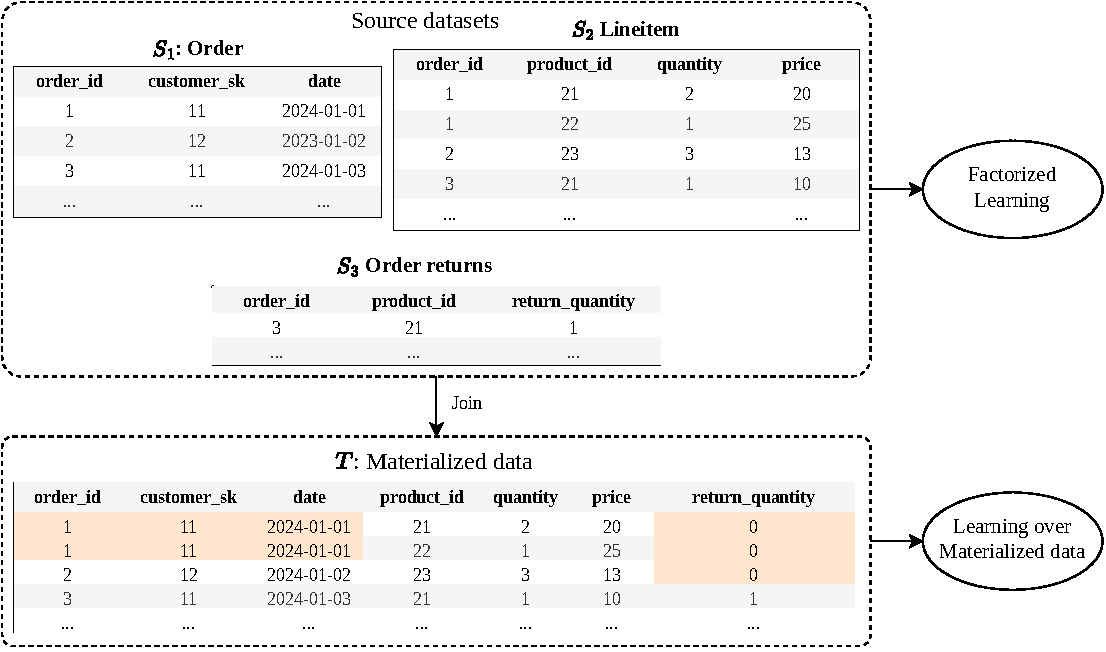
\includegraphics[width=0.95\linewidth]{chapters/01_introduction/figures/running-example-intro.pdf}
    \caption{Illustration of input data used for Factorized Learning vs. Learning over Materialized data, schema from TPCx-AI \cite{tpcx_ai} Use Case 1 (unused columns not shown). Target redundancy avoided by factorization shown in orange.}
    \label{fig:running-example-fac-vs-mat}
\end{figure}

When a data scientist wants to train an ML model, they first need to join disparate sources to create a single dataset (Materialization \cite{rel_db_glossary}) to use as input for an ML model. Factorized Learning eliminates this step in the training process by learning directly from the source datasets, without first joining them. \autoref{fig:running-example-fac-vs-mat} illustrates the difference between factorized learning and learning over materialized data. The reason that factorized learning can be more efficient is that values in the materialized data (orange cells in $T$ in the figure) do not lead to redundant computations during training. However, the source datasets can also have redundant values, and this redundancy is not the only factor that affects the efficiency of factorized learning. Apart from the data-characteristics (which include redundancy), model parameters and hardware characteristics can also influence the choice between factorized learning and materialization.

Deciding between factorization and materialization is a multi-dimensional cost optimization problem. This is an interesting and important problem because factorized learning is a very novel approach to the fundamentals of machine learning. It has the potential to reduce the cost of model training without affecting performance. It could also be easily extensible to federated learning in a scenario where computation involving a source dataset is executed in the silo that dataset resides in.

However, solving this problem is challenging because the optimization space is exceptionally large and may be hardware dependent. Previous solutions, such as Morpheus \cite{morpheus} and Amalur's cost estimation \cite{schijndel_cost_estimation}, have focused on theoretical cost or simple heuristics without considering the hardware dimension.

\begin{figure}[h]
    \centering
    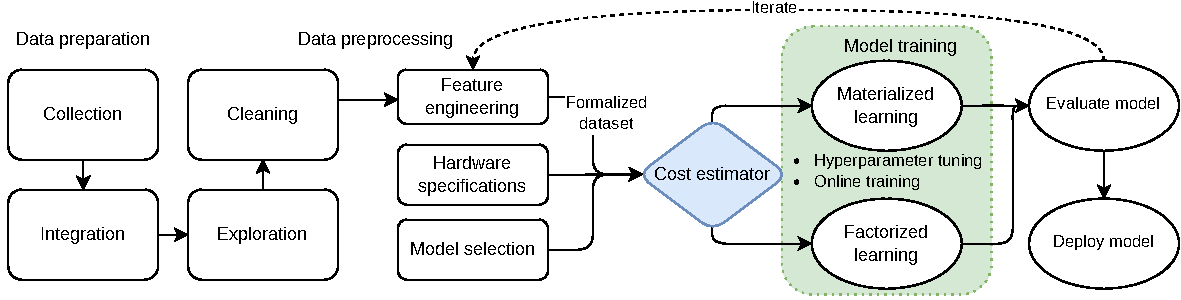
\includegraphics[width=0.95\linewidth]{chapters/01_introduction/figures/ML-Pipeline.pdf}
    \caption{Function of this thesis' cost estimator in an ML pipeline.}
    \label{fig:ml-pipeline}
\end{figure}

\autoref{fig:ml-pipeline} shows the applicability of the cost estimator we propose. For an ML practitioner aiming to optimize their training processes with the use of factorized learning, the data preparation and preprocessing steps do not change. They will still need to gather source datasets and define how to e.g., join and clean them. After they have finished preprocessing, formalized how the datasets should be joined, and decided what model they want to train, the cost estimator predicts the optimal training method. Utilizing such a cost estimator can result in considerable time savings in intensive training scenarios, such as hyper-parameter tuning or training complex models.


\section{Research Questions \& Contributions}
This thesis focuses on facilitating the adoption of factorized machine learning by developing a model that can accurately decide the optimal approach (from factorized and materialized computation), for training a machine learning model, considering the data, model and hardware dimensions.

\subsection{Research Questions}
The research questions answered in this thesis are:
\begin{itemize}
    \item[RQ.1] How can we optimize and implement Factorized Machine Learning for GPUs?
    \item[RQ.2] How can we accurately predict the optimal choice between factorized or materialized training of a Machine Learning model, on CPU and GPU, through leveraging knowledge about model, data, and hardware characteristics?
\end{itemize}

\subsection{Contributions}
\begin{enumerate}
    \item[C.1] A GPU optimized implementation of Amalur's Factorized Machine Learning framework.
    \item[C.2] A cost model that predicts whether factorized or materialized learning is faster, capable of accurate predictions regardless of dataset, model hyper-parameters, or hardware used. This cost model is the result of a detailed study comparing multiple cost calculation strategies.
\end{enumerate}

\section{Running Example}
\todo{formalization of the running example
    \begin{itemize}
        \item Usecase
        \item schema
        \item more details
    \end{itemize}
}

\section{Cost Estimation for Factorized Machine Learning}
To develop a cost estimator that can accurately predict whether Factorized or materialized learning is faster for a given ML task we conduct experiments on synthetic data allowing for full control of the relevant data, model and hardware factors. These empirical where then used results to train several models. We compare these models with each other, as well as with multiple baselines from related works. This was done not only to show which models performs best, but to also create thorough understanding on why these models perform the way they do.

Evaluation on real-world datasets show that our models outperform the state-of-the-art, specifically the \textbf{???} model performs well. It performs \textbf{???} as well as state-of-the-art Amalur \cite{schijndel_cost_estimation} on Hamlet datasets \cite{2016hamletsigmod}. It also performed well on the TPC-AI use cases, saving \textbf{???}\% of training time over a system without factorized ML and a cost estimator to decide whether to do materialized or factorized computation. The goal of creating a generalizable model, one that still has accurate prediction capabilities even if the scenario under evaluation is not similar to one the model was trained on, was also achieved. The final estimator only loses \textbf{???} of its predictive power on use cases with hardware, and data characteristics not in its training set.
% Something more about why this model performs the best


\section{Outline}
This section provides an overview of the structure for the rest of this thesis. We start with the theoretical concepts and principles that underpin our study in \autoref{chapter:preliminary}. The literature review (\autoref{chapter:literature}) surveys existing research relevant to our topic and identifies gaps or limitations in the existing literature. In the \hyperref[chapter:methodology]{methodology chapter}, we describe our overall approach to this empirical study, including the breakdown and motivation for the chosen independent variables. The experiment setup in \autoref{chapter:experiment-setup} provides a detailed description of the experimental environment, as well as the necessary information to replicate the results shown after. In the next chapter on \hyperref[chapter:cost-estimations]{cost estimation} we detail the statistical and analytical methods used to analyze the data, present the results of each experiment, and include visualizations to illustrate key findings. The \hyperref[chapter:evaluation-discussion]{evaluation \& discussion chapter} discusses the outcomes of the experiments in relation to the research questions, evaluates the validity and reliability of the results, compares our findings with existing literature, and provides an in-depth interpretation of the results. We also discuss the practical implications of our findings and acknowledge any limitations of our study. Finally, in the conclusion chapter (\autoref{chapter:conclusion}), the main main contributions and findings of this thesis are summarized, and we provide an outlook for future research.


%! TEX root = ../../main.tex

\chapter{Preliminaries: Factorized Machine Learning}
\label{chapter:preliminary}

This chapter details the preliminary theoretical concepts for this thesis. First, we explain \hyperref[sec:2-data-integration]{Data Integration}: the process of combining data from different sources, which is crucial for any ML workflow. With these concepts in mind, we explore \hyperref[sec:2-factorized-ml]{Factorized Machine Learning} in detail. Finally, in \autoref{sec:2-ml-on-gpu}, we explain GPUs and how they are crucial for the ML industry. With these concepts, we provide the theoretical foundation necessary for understanding the content presented in the next chapters of this thesis.


\section{Data Integration}
\label{sec:2-data-integration}
In order to comprehend the significance and complexities of Factorized Machine Learning (ML), it is necessary to have a grasp of the field of Data Integration (DI). In its broadest sense, DI details the relationships between datasets, enabling the merging of data from diverse sources into a unified dataset. This process is crucial for ML applications, as ML frameworks (such as Keras\footnote{\url{https://keras.io/}} and TensorFlow\footnote{\url{https://www.tensorflow.org/}}) typically require a single table as input. An example of such a DI scenario is illustrated in \autoref{fig:running-example-fac-vs-mat}.

However, when merging data sets into a unified table is essential for machine learning, it may present the following significant challenges \cite{data-management-in-ML-kumar-2017}.

\begin{enumerate}
    \item \textbf{Extra storage}\\ The joined dataset will take extra space to store.
    \item \textbf{Computational redundancy} \\ Joining tables can introduce duplication of values in the materialized data (shown in orange in \autoref{fig:running-example-fac-vs-mat}). These values are included in any computations made during the training of an ML model in this dataset, resulting in duplicate computations.
    \item \textbf{Join time} \\For complex scenarios, joining datasets can take a significant amount of time.
    \item \textbf{Maintenance headaches} \\Join query needs updating when changing input table schemas.
\end{enumerate}

Factorized Machine Learning seeks to address issues one through three through the concept of ``learning over joins'' \cite{orion_learning_gen_lin_models}, which involves shifting the computations required for an ML model to the individual tables.

\subsection{Schema Mapping}
Schema mapping is an integral step in the Data Integration process and thus to Factorized ML. These mappings specify how the source datasets map to the target tables. Having a formal way to specify how these datasets relate is especially important for factorized ML. It allows us to convert these relationships between the source tables and the target table to a form that can be translated to linear algebra: the normalized matrix (detailed in \autoref{subsec:2-normalized-matrix}).

The language used for these mappings is \textit{source-to-target tuple generating dependencies (s-t tgd)} \cite{tgds-Fagin2009}. These are first-order logic formulas that specify, through atomic formulas over schemas $S$ and the target schema $T$, how the tuples of the source tables map to the target table. Here, we show the TGD for the running example.\begin{alignat*}{2}
    \intertext{Given source datasets, with abbreviated column names:}
     & o=order\_id, c=customer\_id, d=date,                                                                                                                      \\
     & p_{id}=product\_id, q=quantity, p=price, rq=return\_quantity                                                                                              \\
     & S_1(o, c, d)                                                                                                                                              \\
     & S_2(o, p_{id} , q,  p)                                                                                                                                    \\
     & S_3(o, p_{id}, rq)                                                                                                                                      & \\
    \intertext{the mapping to target table $T$ can be specified as follows. First, we left join $S_2$ with $S_3$:}
     & \forall o, p_{id}, q, p, rq \left( S_3(o, p_{id}, rq) \land S_2(o, p_{id}, q, p) \rightarrow \exists o, p_{id}, q, p, rq T(o, p_{id}, q, p, rq) \right)   \\
    \intertext{Next, we inner join the result with $S_1$ to get the final schema $T(o, c, d, p_{id}, q, p, rq)$:} \begin{split}
                                                                                                                      & \forall o, c, d, p_{id}, q, p, rq ( S_1(o, c, d) \land T(o, p_{id}, q, p, rq) \rightarrow \\
                                                                                                                      & \exists o, c, d, p_{id}, q, p, rq T(o, c, d, p_{id}, q, p, rq) )
                                                                                                                  \end{split}
\end{alignat*}

Now that we have the schema mapping we can translate this to the normalized matrix, which we will do in the next section.

\section{Factorized Machine Learning}
\label{sec:2-factorized-ml}
As stated previously in this thesis, Factorized ML is the process of training Machine Learning models on multiple tables without the need to materialize the join between these tables. This section will go in-depth on how this can be achieved, continuing the running example from \autoref{fig:running-example-fac-vs-mat}.  We start with the definitions (\autoref{subsec:2-normalized-matrix}) followed by an in-depth example of the involved linear algebra (\autoref{subsubsec:2-fac-ml-example}).

\subsection{Normalized Matrix}
\label{subsec:2-normalized-matrix}
As Machine Learning algorithms can be expressed in Linear Algebra (LA), we need to express the Data Integration scenario of an ML use case in terms of Linear Algebra, .i.e., we need to translate the Schema Mappings of an integration scenario to Linear Algebra to allow us to achieve the goal of “pushing down” ML to the separate source tables. This is achieved through the \textbf{Normalized matrix}: A set of matrices that capture the necessary DI metadata telling us how the source tables map to the materialized Target table \cite{amalur, morpheus}.

The \textbf{Mapping matrix} and \textbf{Indicator matrix} respectively represent how the columns and rows from each source table $S_k$ map to the Target table $T$.

\subsubsection{Mapping Matrix}
The Mapping Matrix $M$ is a set of matrices $M_k$ for each source table $S_k$ that denotes how source columns map to target columns. A value of 1 in this matrix indicates that the corresponding column (via column number) in $S_k$ corresponds to the corresponding column (via column number) in $T$. The formal definition is as follows.

\begin{definition}[\textit{Mapping matrix} \cite{amalur}]
    Each source table $S_k$ has a corresponding binary Mapping matrix $M$ of shape $c_T \times c_{S_k}$, where
    \begin{align*}
        M_k[i,j] = \begin{cases}
                       1, & \text{if $j$-th column of $S_k$ is mapped to the $i$-th column of $T$} \\
                       0, & \text{otherwise}
                   \end{cases}
    \end{align*}
\end{definition}

Note that in the case that there is no column overlap between source tables this Mapping Matrix is redundant. This affects the materialization step, as shown in \autoref{def:materialization}.


\subsubsection{Indicator Matrix}
Now that we have defined how to map the columns from the source tables to the target table, we need to do the same for the rows. This is done with the \textbf{Indicator} matrix.

\begin{definition}[\textit{Indicator matrix} \cite{morpheus}]
    Each source table $S_k$ has a corresponding binary Indicator matrix $I$ of shape $r_T \times r_{S_k}$, where
    \begin{align*}
        I_k[i,j] = \begin{cases}
                       1, & \text{if $i$-th row of $S_k$ is mapped to the $j$-th row of $T$} \\
                       0, & \text{otherwise}
                   \end{cases}
    \end{align*}
\end{definition}

\subsubsection{Materialization}
Using the normalized matrix, we can now \textbf{materialize} the join to obtain the target matrix $T$:

\begin{definition}[\textit{Materializing the Normalized Matrix to obtain Target matrix $T$}]
    \begin{itemize}
        \item[]
        \item[] Given
        \item[$k$] Table id $k \in [1,n]$
        \item[$S_k$] Source tables
        \item[$M_k$] Mapping matrices
        \item[$I_k$] Indicator matrices
    \end{itemize}
    \[
        T = \begin{cases}
            \sum_{k=1}^n  I_k S_k M^T_k,  & \text{if there is column overlap between source tables} \\
            \begin{bNiceMatrix}
                \vdots  & \vdots & \vdots  \\
                I_1 S_1 & \cdots & I_n S_n \\
                \vdots  & \vdots & \vdots  \\
            \end{bNiceMatrix}, & \text{otherwise}
        \end{cases}
    \]
    \label{def:materialization}

\end{definition}

The materialization case when there is no column overlap is a horizontal concatenation of each source matrix $S_k$ multiplied by $I_k$: $I_k S_k, k \in [1,n]$. Intuitively the materialization process can be seen as:
\begin{algorithmic}
    \ForEach {$k \in [1,n]$} \Comment{For each source table}
    \State $rows_k \gets I_k S_k$ \Comment{Map the source table rows to the target table}
    \State $T_k \gets rows_k M^T_k$ \Comment{Map the source table columns to the target table}
    \EndFor
    \State $T \gets \sum_{k=1}^{n} T_k$ \Comment{Sum the results}
\end{algorithmic}

\subsubsection{Running Example: Normalized Matrix}
\label{subsubsec:2-fac-ml-example}
To translate the normalized matrix to how it is used in ML algorithms, we first show the full normalized matrix of the running example, followed by the materialized Target table $T$. The goal is to show how the matrices interact to allow computation with all information without necessarily materializing the join. For completeness, we show the calculations with the Mapping matrices $M_k$ included, but as highlighted before, this is not needed due to this scenario having no column overlap. However, it is insightful to show as it gives an idea of how this process looks when there is column overlap.
\begin{alignat*}{6}
    \intertext{
        These are the corresponding Source matrices $S_{1..3}$ for the source tables shown in \autoref{fig:running-example-fac-vs-mat}. The \textcolor{BurntOrange}{orange} numbers over the columns denote in which column of $T$ they will end up. The \textcolor{RoyalBlue}{blue} numbers at the end of each row illustrate to which target table rows they are mapped.
    }
                                                            & S_1 &     & =
    \begin{bNiceMatrix}[first-row,last-col]
        0 & 1  & 2    &     \\
        1 & 11 & 2024 & 0,1 \\
        2 & 12 & 2024 & 2   \\
        3 & 11 & 2024 & 3   \\
    \end{bNiceMatrix}   \quad                 &     & S_2 &   & =
    \begin{bNiceMatrix}[first-row,last-col]
        3 & 4  & 5  &   \\
        2 & 20 & 40 & 0 \\
        1 & 25 & 25 & 1 \\
        3 & 13 & 39 & 2 \\
        1 & 10 & 10 & 3 \\
    \end{bNiceMatrix}           \quad                 &     & S_3 &   & =
    \begin{bNiceMatrix}[first-row,last-col]
        6 &   \\
        1 & 3 \\
    \end{bNiceMatrix}                                  \\
    \intertext{
        The Indicator matrices denote how rows from $S$ map to rows in $T$. The column number denotes the row in $S$, the row number denotes the row in $T$. The \textcolor{RoyalBlue}{blue} annotations show more clearly how this works in the form \textcolor{RoyalBlue}{row number in $S_k \rightarrow$ row number in $T$}.
    }
                                                            & I_1 &     & =
    \begin{bNiceMatrix}[last-col]
        1 & 0 & 0 & 0 \rightarrow 0 \\
        1 & 0 & 0 & 0 \rightarrow 1 \\
        0 & 1 & 0 & 1 \rightarrow 2 \\
        0 & 0 & 1 & 2 \rightarrow 3 \\
    \end{bNiceMatrix}   \quad                          &     & I_2 &   & =
    \begin{bNiceMatrix}[last-col]
        1 & 0 & 0 & 0 & 0 \rightarrow 0 \\
        0 & 1 & 0 & 0 & 1 \rightarrow 1 \\
        0 & 0 & 1 & 0 & 2 \rightarrow 2 \\
        0 & 0 & 0 & 1 & 3 \rightarrow 3 \\
    \end{bNiceMatrix}     \quad                      &     & I_3 &   & =
    \begin{bNiceMatrix}[last-col]
        0 & \rightarrow 0   \\
        0 & \rightarrow 1   \\
        0 & \rightarrow 2   \\
        1 & 0 \rightarrow 3 \\
    \end{bNiceMatrix}                                            \\
    \intertext{
        The Mapping matrices denote how columns from $S$ map to columns in $T$. The row number denotes the column in $T$, the column number denotes the column in $S$. The \textcolor{BurntOrange}{orange} annotations show this in the form: \textcolor{BurntOrange}{column number in $S_k \rightarrow$ column number in $T$}.
    }
                                                            & M_1 &     & =
    \begin{bNiceMatrix}[last-col]
        1 & 0 & 0 & \textcolor{BurntOrange}{0 \rightarrow 0} \\
        0 & 1 & 0 & \textcolor{BurntOrange}{1 \rightarrow 1} \\
        0 & 0 & 1 & \textcolor{BurntOrange}{2 \rightarrow 2} \\
        0 & 0 & 0 & \textcolor{BurntOrange}{\rightarrow 3}   \\
        0 & 0 & 0 & \textcolor{BurntOrange}{\rightarrow 4}   \\
        0 & 0 & 0 & \textcolor{BurntOrange}{\rightarrow 5}   \\
        0 & 0 & 0 & \textcolor{BurntOrange}{\rightarrow 6}   \\
    \end{bNiceMatrix}   \quad &     & M_2 &   & =
    \begin{bNiceMatrix}[last-col]
        0 & 0 & 0 & \textcolor{BurntOrange}{\rightarrow 0}   \\
        0 & 0 & 0 & \textcolor{BurntOrange}{\rightarrow 1}   \\
        0 & 0 & 0 & \textcolor{BurntOrange}{\rightarrow 2}   \\
        1 & 0 & 0 & \textcolor{BurntOrange}{0 \rightarrow 3} \\
        0 & 1 & 0 & \textcolor{BurntOrange}{1 \rightarrow 4} \\
        0 & 0 & 1 & \textcolor{BurntOrange}{2 \rightarrow 5} \\
        0 & 0 & 0 & \textcolor{BurntOrange}{\rightarrow 6}   \\
    \end{bNiceMatrix} \quad &     & M_3 &   & =
    \begin{bNiceMatrix}[last-col]
        0 & \textcolor{BurntOrange}{\rightarrow 0}   \\
        0 & \textcolor{BurntOrange}{\rightarrow 1}   \\
        0 & \textcolor{BurntOrange}{\rightarrow 2}   \\
        0 & \textcolor{BurntOrange}{\rightarrow 3}   \\
        0 & \textcolor{BurntOrange}{\rightarrow 4}   \\
        0 & \textcolor{BurntOrange}{\rightarrow 5}   \\
        1 & \textcolor{BurntOrange}{0 \rightarrow 6} \\
    \end{bNiceMatrix}
\end{alignat*}
\begin{gather*}
    \begin{alignat*}{4}
        \intertext{For conciseness we show the calculation of one of the sub-target tables $T_1$.}
                            & T_1 &       & = I_1                 &  & S_1 &  & M_1^T                   \\
                            & T_1 &       & = \begin{bNiceMatrix}
                                                  1 & 0 & 0 \\
                                                  1 & 0 & 0 \\
                                                  0 & 1 & 0 \\
                                                  0 & 0 & 1 \\
                                              \end{bNiceMatrix} &  &
        \begin{bNiceMatrix}
            1 & 11 & 2024 \\
            2 & 12 & 2024 \\
            3 & 11 & 2024 \\
        \end{bNiceMatrix} &     & M_1^T                                                                 \\
                            & T_1 &       & = \begin{bNiceMatrix}
                                                  1 & 11 & 2024 \\
                                                  1 & 11 & 2024 \\
                                                  2 & 12 & 2024 \\
                                                  3 & 11 & 2023 \\
                                              \end{bNiceMatrix} &  &     &  & \begin{bNiceMatrix}
                                                                                  1 & 0 & 0 & 0 & 0 & 0 & 0 \\
                                                                                  0 & 1 & 0 & 0 & 0 & 0 & 0 \\
                                                                                  0 & 0 & 1 & 0 & 0 & 0 & 0 \\
                                                                              \end{bNiceMatrix} \\
    \end{alignat*}\\
    \hspace{-4cm}
    T_1  = \begin{bNiceMatrix}
        \Block[fill=red!15,rounded-corners]{4-3}{}
        1 & 11 & 2024 & 0 & 0 & 0 & 0 \\
        1 & 11 & 2024 & 0 & 0 & 0 & 0 \\
        2 & 12 & 2024 & 0 & 0 & 0 & 0 \\
        3 & 11 & 2023 & 0 & 0 & 0 & 0 \\
    \end{bNiceMatrix}
\end{gather*}

\begingroup
\setlength{\arraycolsep}{4.5pt}
\begin{alignat*}{2}
    \intertext{
        The materialized Target table $T$ is the element wise sum of the dot product of each tuple of Indicator, Source, and Mapping matrices. For each source table $S_k$ the intermittent result is shown as $T_k$. For clarity the cells from each source table are coloured in the same colour in the intermittent result and in Target table $T$.
    }
     & T_1= I_1 S_1 M_1^T &  & = \begin{bNiceMatrix}[first-row]
                                     0 & 1  & 2    & 3 & \cdots & 6 \\
                                     \Block[fill=red!15,rounded-corners]{4-3}{}
                                     1 & 11 & 2024 & 0 & \cdots & 0 \\
                                     1 & 11 & 2024 & 0 & \cdots & 0 \\
                                     2 & 12 & 2024 & 0 & \cdots & 0 \\
                                     3 & 11 & 2023 & 0 & \cdots & 0 \\
                                 \end{bNiceMatrix}
    T_2= I_2 S_2 M_2^T= \begin{bNiceMatrix}[first-row]
                            0 & 1 & 2 & 3                                             & 4  & 5  & 6 \\
                            0 & 0 & 0 & \Block[fill=blue!15,rounded-corners]{4-3}{} 2 & 20 & 40 & 0 \\
                            0 & 0 & 0 & 1                                             & 25 & 25 & 0 \\
                            0 & 0 & 0 & 3                                             & 13 & 39 & 0 \\
                            0 & 0 & 0 & 1                                             & 10 & 10 & 0 \\
                        \end{bNiceMatrix}
    \\
     & T_3= I_3 S_3 M_3^T &  & = \begin{bNiceMatrix}[first-row]
                                     0 & \cdots & 5 & 6                                              \\
                                     0 & \cdots & 0 & 0                                              \\
                                     0 & \cdots & 0 & 0                                              \\
                                     0 & \cdots & 0 & 0                                              \\
                                     0 & \cdots & 0 & \Block[fill=orange!15,rounded-corners]{1-1}{}1 \\
                                 \end{bNiceMatrix}
    T  = \sum_{k=1}^{3} I_k S_k M^T_k =  \begin{bNiceMatrix}[first-row,last-col]
                                             0 & 1  & 2    & 3                                           & 4  & 5  & 6                                                  \\
                                             \Block[fill=red!15,rounded-corners]{4-3}{}
                                             1 & 11 & 2024 & \Block[fill=blue!15,rounded-corners]{4-3}{}
                                             2 & 20 & 40   & 0                                           & 0                                                            \\
                                             1 & 11 & 2024 & 1                                           & 25 & 25 & 0                                              & 1 \\
                                             2 & 12 & 2024 & 3                                           & 13 & 39 & 0                                              & 2 \\
                                             3 & 11 & 2024 & 1                                           & 10 & 10 & \Block[fill=orange!15,rounded-corners]{1-1}{}1 & 3 \\
                                         \end{bNiceMatrix}
\end{alignat*}
\endgroup


\subsection{Factorized Linear Algebra}
In the previous section, we have shown the properties of the Normalized matrix. This section will show how commonly used Linear Algebra operators are rewritten for the Normalized matrix for the purpose of performing factorized ML \cite{morpheus}. We will show how to perform element-wise operations, reduction operations, dot-product operations, and a running example of right matrix multiplication (RMM) on the Normalized matrix. The goal is to show how (most of) these operations can be performed without materializing the join between the source tables, and how the Normalized matrix allows us to do so.


\subsubsection{Element-wise Scalar Operations}
This group of operators perform an operation on every element of a matrix independently of each other. The arithmetic operations are: $+$, $-$, $\times$, $\div$ and $ ^\wedge $ (these operators are denoted by $\oslash$). This can be seen as a scalar function $f$ applied to each element of a matrix $T$. The rewrite rule therefore is very simple for these arithmetic operators, as well as for any other scalar function (e.g., $log$, $round$) $f$:
\begin{alignat*}{2}
    x \oslash T & \rightarrow [x \oslash S, I, M] \\
    T \oslash x & \rightarrow [S \oslash x, I, M]
    \intertext{or more generally:}
    f(T)        & \rightarrow [f(S), I, M]
\end{alignat*}

These operations all return a normalized matrix and can thus be performed without materializing the join between the source tables. In the used implementation \cite{schijndel_cost_estimation}, when a normalized matrix is transposed, the actual computation is not carried out, but the transpose is simply added as a flag. Then, for any downstream operators, the transpose flag is checked, and the computation is performed accordingly. For these element-wise operations the transposed rewrite is:
\begin{alignat*}{2}
    f(T^T) & \rightarrow [f(S), I, M]^T
\end{alignat*}

\subsubsection{Aggregation}
The supported aggregation operators are row-wise and column-wise summation, respectively abbreviated to rowSums and colSums. For the factorized rowSums case we sum each source table separately, then multiply with the indicator matrices and sum the results, the mapping matrix is irrelevant. This operation produces a single (column) vector of size $r_T \times 1$. For the transposed case, it is equal to a column summation. These rewrite rules are:
\begin{alignat*}{2}
    \text{rowSums}(T)   & \rightarrow \sum_{k=1}^n I_k \text{rowSums}(S_k) \\
    \text{rowSums}(T^T) & \rightarrow \text{colSums}(T)
\end{alignat*}

Summing column-wise gives a row vector of shape $1 \times c_T$. It is equal to first summing the indicator tables column-wise, then materializing with these aggregated indicator matrices.  The rewrite rule for the factorized case is:
\begin{alignat*}{2}
    \text{colSums}(T)   & \rightarrow \sum_{k=1}^n \text{colSums}(I_k) S_k M_k^T \\
    \text{colSums}(T^T) & \rightarrow \text{rowSums}(T)
\end{alignat*}
As these operations do not create normalized matrices, and in fact materialize (part of) the join the benefit of factorized computation is smaller.

\subsubsection{Multiplication}
As matrix multiplication is not commutative, there are different rewrite rules for left- and right-matrix multiplication. The rewrite rule for left matrix multiplication (LMM) with another matrix $X$ is:
\begin{alignat*}{2}
    TX   & \rightarrow \sum_{k=1}^n I_k S_k M_k^T X \\
    T^TX & \rightarrow (X^TT)^T
\end{alignat*}

For right matrix multiplication (RMM) the rule is the same, we still essentially materialize the join, but with $X$ on the left-hand side:
\begin{alignat*}{2}
    XT   & \rightarrow \sum_{k=1}^n X I_k S_k M_k^T \\
    XT^T & \rightarrow (TX^T)^T
\end{alignat*}

\subsubsection{Running Example: Right Matrix Multiplication}

\begingroup
\setlength{\arraycolsep}{3.0pt}
\begin{alignat*}{1}
    \intertext{We showcase right RMM and its rewrite rule by multiplying with $X$. First for the materialized Target table $T$:}
    X T & = \begin{bNiceMatrix}
                1 & 1 & 2 & 3 \\
            \end{bNiceMatrix}
    \begin{bNiceMatrix}
        1 & 11 & 2024 & 2 & 20 & 40 & 0 \\
        1 & 11 & 2024 & 1 & 25 & 25 & 0 \\
        2 & 12 & 2024 & 3 & 13 & 39 & 0 \\
        3 & 11 & 2023 & 1 & 10 & 10 & 1 \\
    \end{bNiceMatrix}                                                         \\
        & =\begin{bNiceMatrix}
               15 & 79 & 14165 & 12 & 101 & 173 & 3 \\
           \end{bNiceMatrix}                                             \\
    \intertext{Now for the Normalized matrix, recall the rewrite rule for RMM:}
    X T & = \sum_{k=1}^{n} X I_k S_k M^T_k
    \intertext{For conciseness we refer back to sub results $T_{0\cdots2}$ and use them directly here. We also leave out $X$ in the subcalculations for $T_{1,2}$.}
        & = X T_0 + X T_1 + X T_2                                                           \\
        & = \begin{bNiceMatrix}
                1 & 1 & 2 & 3 \\
            \end{bNiceMatrix} \begin{bNiceMatrix}
                                  1 & 11 & 2024 & 0 & \cdots & 0 \\
                                  1 & 11 & 2024 & 0 & \cdots & 0 \\
                                  2 & 12 & 2024 & 0 & \cdots & 0 \\
                                  3 & 11 & 2023 & 0 & \cdots & 0 \\
                              \end{bNiceMatrix} + X \begin{bNiceMatrix}
                                                        0 & 0 & 0 & 2 & 20 & 40 & 0 \\
                                                        0 & 0 & 0 & 1 & 25 & 25 & 0 \\
                                                        0 & 0 & 0 & 3 & 13 & 39 & 0 \\
                                                        0 & 0 & 0 & 1 & 10 & 10 & 0 \\
                                                    \end{bNiceMatrix} + X\begin{bNiceMatrix}
                                                                             0 & \cdots & 0 & 0 \\
                                                                             0 & \cdots & 0 & 0 \\
                                                                             0 & \cdots & 0 & 0 \\
                                                                             0 & \cdots & 0 & 1 \\
                                                                         \end{bNiceMatrix} \\
        & =\begin{bNiceMatrix}
               15 & 79 & 14165 & 0 & 0 & 0 & 0 \\
           \end{bNiceMatrix} +
    \begin{bNiceMatrix}
        0 & 0 & 0 & 12 & 101 & 173 & 0 \\
    \end{bNiceMatrix}+
    \begin{bNiceMatrix}
        0 & 0 & 0 & 0 & 0 & 0 & 3 \\
    \end{bNiceMatrix}                                                               \\& =\begin{bNiceMatrix}
        15 & 79 & 14165 & 12 & 101 & 173 & 3 \\
    \end{bNiceMatrix}
\end{alignat*}
\endgroup

\subsection{Machine Learning Models}
We use the same machine learning models as Morpheus \cite{morpheus} and \cite{schijndel_cost_estimation}. These models consist of Linear Regression, Logistic Regression, K-means clustering, and Gaussian NMF. Having demonstrated the transformation rules for the relevant Linear Algebra operations, we are now able to illustrate how these models can be adapted for the Normalized matrix. This adaptation enables us to execute these machine learning models without materializing the join between the source tables. The algorithms are detailed in the next sections, with the factorized operators used highlighted in red. Within the algorithms, we use the following conventions: $X$ represents the matrix of independent variables, which in our scenario corresponds to the normalized matrix. The dependent variable is denoted as $y$, the weight vector as $w$, the learning rate as $\gamma$, and $n$ represents the number of iterations.

\subsubsection{Linear Regression}
\begin{algorithm}[ht!]
    \caption[Linear regression]{Linear regression using Gradient Descent
        \cite{morpheus}}\label{alg:linear-regression}
    \begin{algorithmic}
        \Require $X, y , w, \gamma$
        \For{$i \in 1:n$}
        \State $w = w - \gamma (\text{\red{$X^T$}}((\text{\red{$X w$}}) - y))$
        \EndFor
    \end{algorithmic}
\end{algorithm}
Linear Regression (\autoref{alg:linear-regression}) is an ML technique fit to find linear relationships between independent variables and a dependent variable. The algorithm utilises gradient descent to iteratively converge towards the best solution. The LA operators performed on the normalized matrix $T$ are Transpose $T^T$, and Left Matrix Multiplication $TX$.

\subsubsection{Logistic Regression}
Logistic Regression (\autoref{alg:logistic-regression}) is very similar to Linear Regression, but instead of predicting a continuous value, it predicts a binary value. The rewrite rule for Logistic Regression uses the same operators as Linear Regression: Transpose and Left Matrix Multiplication.

\begin{algorithm}[ht]
    \caption[Linear regression]{Logistic regression using Gradient Descent
        \cite{morpheus}}\label{alg:logistic-regression}
    \begin{algorithmic}
        \Require $X, y , w, \gamma$
        \For{$i \in 1:n$}
        \State $w = w - \gamma \left(\text{\red{$X^T$}} \frac{y}{1+e^{\text{\red{$X w$}}}}\right)$
        \EndFor
    \end{algorithmic}
\end{algorithm}

\subsubsection{K-means Clustering}
The regression algorithms discussed above are supervised, that is, they predict a value based on a set of input features. K-means clustering is an unsupervised algorithm that groups data points into a predefined number of clusters based on their similarity. The operators used to calculate the clusters are $exp$ ($X^2$), Scalar Multiplication, Transposition, Row Summation, and Left Matrix Multiplication. The algorithm is shown in \autoref{alg:k-means}.

\begin{algorithm}[ht]
    \caption[K-Means Clustering]{K-Means Clustering
        \cite{morpheus}\\
        $\mathbf{1}_{r \times c}$ denotes a matrix of size $r \times c$ filled with ones, this is used to repeat a vector to a matrix, either row- or column-wise.}\label{alg:k-means}
    \begin{algorithmic}
        \Require $X, k$ (number of centroids)
        \State $C = \text{rand}(r_X \times k)$ \Comment{Randomly initialize centroids matrix $C$}
        \State $D_X = \text{\red{rowSums($X^2$)}} \times \mathbf{1}_{1 \times k}$ \Comment{Compute the $l^2$-norm of points for distances}
        \State $T_2 = \text{\red{$2 \times X$}}$

        \For{$i \in 1:n$}
        \State $D = D_X - T_2C + \left( \mathbf{1}_{r_X\times 1} \times \text{colSums}(C^2) \right)$ \Comment{Compute distances}
        \State $A = (D == \text{rowMin}(D) \times \mathbf{1}_{1 \times k})$ \Comment{Assign points to the closest centroid}
        \State $C =\frac{\text{\red{$X^T A$}}}{\mathbf{1}_{c_X \times 1} \times \text{colSums}(A)}$ \Comment{Update centroids}
        \EndFor
    \end{algorithmic}
\end{algorithm}

\subsubsection{Gaussian Non-negative Matrix Factorization}
Gaussian Non-negative Matrix Factorization (Gaussian NMF) is a technique used to decompose a matrix into two smaller nonnegative matrices. It is used for feature extraction from data and is often used in image processing and text mining. The operators used in the algorithm are Transpose and Right Matrix Multiplication. The rank hyperparameter $r$ controls the size of the resulting matrices. The algorithm is shown in \autoref{alg:gaussian-nmf}.

\begin{algorithm}[ht]
    \caption[Gaussian NMF]{Gaussian Non-negative Matrix Factorization
        \cite{morpheus}}\label{alg:gaussian-nmf}
    \begin{algorithmic}
        \Require $X, r\ \text{(rank)}$
        \State $W = \text{rand}(r_X \times r)$ \Comment{Randomly initialize $W$}
        \State $H = \text{rand}(r \times c_X)$ \Comment{Randomly initialize $H$}
        \For{$i \in 1:n$}
        \State $H = H \times \left(\frac{\text{\red{$W^T X$}}}{W^T W H}\right)$
        \State $W = W \times \left(\frac{\text{\red{$X H^T$}}}{W(H H^T)}\right)$
        \EndFor
    \end{algorithmic}
\end{algorithm}


\subsection{Overview}
\label{subsec:factorized-ml-summary}
In this section we have presented the rewrite rules for the Normalized matrix, for commonly used Linear Algebra operators, and how these are used in the training of Machine Learning models without the need to explicitly compute the join between the source tables. \autoref{tab:factorized-ml-operators-overview}  provides a summary of the operators discussed, with the final column describing the specific operators employed for each ML model. This underscores the importance of a robust cost model in factorized ML, since various models leverage a range of operators in distinct ways when benefiting from factorized computation.

\begin{table}[ht]
    \small
    \resizebox{\textwidth}{!}{%
        % LTeX: enabled=false
\begin{tabular}{p{0.12\linewidth}p{0.16\linewidth}p{0.1\linewidth}p{0.13\linewidth}p{0.15\linewidth}p{0.19\linewidth}}
\toprule
Group & Operator & Example & 2\textsuperscript{nd} Operand & Output & Used in models \\
\midrule\midrule
\multirow[t]{5}{*}{\parbox{1\linewidth}{\vspace{2.3cm}\hspace{0pt}Element-wise}} & Addition & $T + x$ & scalar $x$ & \multirow[t]{5}{*}{\parbox{1\linewidth}{\vspace{2.3cm}Normalized Matrix}} & — \\

 & Multiplication & $T \times x$ & scalar $x$ &  & K-Means \\

 & Division & $T / x$ & scalar $x$ &  & — \\

 & Transposition & $T^T$ & — &  & LinReg, LogReg, K-Means, G-NMF \\

 & Generic Scalar Function & $f(T)$ & f &  & K-Means ($exp$) \\
\cline{1-6}
\multirow[t]{2}{*}{\parbox{1\linewidth}{\vspace{1.3cm}\hspace{0pt}Aggregation}} & Row Summation & \hspace{0pt} row-Sums$(T)$ & — & Column Vector & K-Means \\

 & Column Summation & \hspace{0pt} col-Sums$(T)$ & — & Row Vector & — \\
\cline{1-6}
\multirow[t]{2}{*}{\parbox{1\linewidth}{\vspace{1.3cm}\hspace{0pt}Multiplication}} & Left Matrix Multiplication & $T Y$ & Matrix Y $(c_T \times r_Y)$ & Matrix $(r_T \times c_X)$ & LinReg, LogReg, K-Means \\

 & Right Matrix Multiplication & $Y T$ & Matrix Y $(c_X \times r_X)$ & Matrix $(r_Y \times c_T)$ & G-NMF \\
\cline{1-6}
\bottomrule
\end{tabular}
}
    \caption{Overview of factorized ML operators.}
    \label{tab:factorized-ml-operators-overview}
\end{table}

\section{Machine Learning on GPUs}
\label{sec:2-ml-on-gpu}
Graphics Processing Units (GPUs) have emerged as the preferred processing units in the Machine Learning domain due to their significant advantages over Central Processing Units (CPUs). As CPUs are designed for diverse general-purpose applications, this is not surprising. Whereas CPUs excel in executing sequential tasks such as running an operating system, GPUs are optimised for parallel tasks. This specialisation enables them to efficiently carry out identical operations on multiple pieces of data simultaneously, exactly what is needed for the prevalent linear algebra operations in ML.

\subsection{Architecture}
\label{subsec:gpu-architecture}

\begin{figure}[ht]
    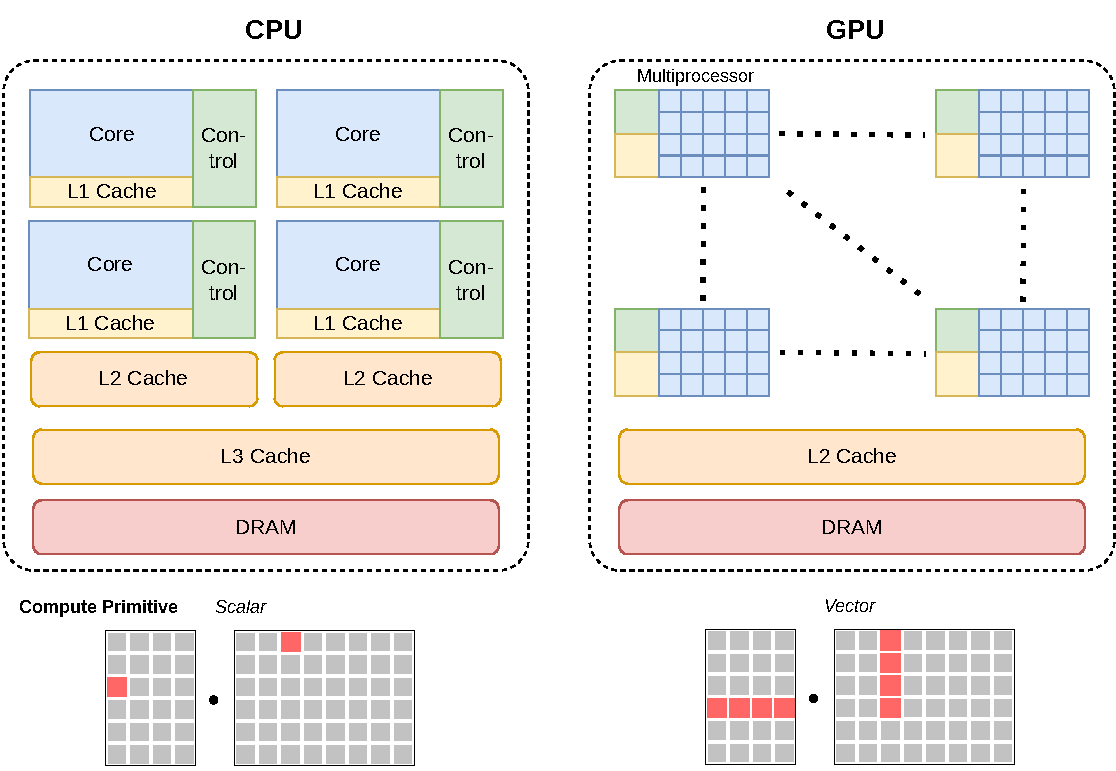
\includegraphics[width=.95\linewidth]{chapters/02_preliminaries/figures/CPU-vs-GPU.pdf}
    \caption[Simplified view of the difference in architecture between a CPU and a GPU.]{ Simplified view of the difference in architecture between a CPU and a GPU. Compute cores are blue, control units green and L1 Cache is marked in yellow. Figure based on visualizations from \cite{gpu-in-ml-survey, cuda-programming-guide, tvm}.}
    \label{fig:cpu-vs-gpu}
\end{figure}
This section elaborates on the architecture of a GPU, emphasizing its effectiveness in performing Linear Algebra tasks. \autoref{fig:cpu-vs-gpu} illustrates the architectural differences between a CPU and a GPU and will serve as a point of reference throughout this section.

The heart of the GPU is the Streaming Multiprocessor (SM), which is responsible for executing thousands of parallel threads. Each SM comprises multiple CUDA cores (highlighted in blue), resembling CPU cores, that carry out arithmetic operations. These cores are optimised to manage multiple operations concurrently, enhancing their effectiveness for the matrix and vector calculations crucial in Machine Learning.

Data and code are transferred to the streaming multiprocessors (SMs) by passing through various memory layers. Initially, data is fetched from the host and stored in the GPU's DRAM, after which it is moved to the SM via the L2 cache. This facilitates quick data exchange and minimises latency. Threads are grouped into blocks and then allocated to SMs for scheduling. This organisation enables efficient resource management and parallel thread execution. Each SM is responsible for managing a block of threads, which are then scheduled for execution. The cores within the SM execute these threads concurrently, resulting in a high degree of parallelism. This simultaneous processing of multiple data points is known as Single Instruction, Multiple Data (SIMD) architecture, which proves to be advantageous in Machine Learning applications, where identical operations are applied across numerous data points. While a CPU can handle a scalar operation within a single clock cycle, a GPU can perform operations on vectors concurrently. This difference in parallelism is illustrated in the lower section of \autoref{fig:cpu-vs-gpu}. 

\subsection{Estimating GPU Performance}
\label{subsec:gpu-performance}
Following the architecture overview, it is essential to grasp the performance dynamics of a GPU in the context of Machine Learning applications, specifically focusing on Linear Algebra operations.. The GPU's ability to execute thousands of threads concurrently is the basis of its computational power, particularly for tasks with high arithmetic intensity. The subsequent passages provide valuable perspectives from \cite{nvidia-gpu-performance:online}.

The arithmetic intensity refers to the ratio of mathematical operations performed per memory operation. In the context of GPUs, it is a critical factor in determining performance constraints. The time it takes for a function to execute on a GPU can be constrained by memory bandwidth, mathematical bandwidth, or latency. To illustrate this, imagine a function that reads the input data, performs calculations, and writes the output. The time spent on memory operations $ T_{mem} $ and math operations $ T_{math} $ can overlap, with the total execution time being the maximum of the two: $ \max(T_{mem}, T_{math})$. Given the inherently sequential nature of CPUs, the total execution time tends to closely approximate the sum of $T_{mem} \text{ and } T_{math}$. This characteristic makes predicting runtime on CPUs more straightforward compared to GPUs, as there are complexities involved in estimating $T_{mem}$ and $T_{math}$ on GPUs.

When the computational time $ T_{math} $ exceeds the memory access time $ T_{mem} $, a function is classified as math-bound, indicating that the GPU's computational capabilities are the limiting factor. In contrast, if $ T_{mem} $ is higher, it is memory-bound, which means that the memory bandwidth is the restricting element. This relationship is illustrated by the inequality $ \frac{\# ops}{BW_{math}} > \frac{\# bytes}{BW_{mem}} $, which can be rearranged as $ \frac{\# ops}{\# bytes} > \frac{BW_{math}}{BW_{mem}} $. Here, the left side denotes a function's arithmetic intensity, while the right side represents the GPU's $ops:byte$ ratio, i.e., the number of Floating Point Operations (FLOPs) per byte retrieved from memory.

In practice, many Machine Learning operations, such as linear layers or activation functions, often have low arithmetic intensities, sometimes executing only one operation for every two-byte element accessed from and stored in memory. This characteristic typically renders them memory-bound on GPUs. However, for operations with high arithmetic intensity, like large matrix multiplications, the GPU's mathematical bandwidth emerges as the constraining factor.

To fully leverage a GPU's capabilities, it is crucial to ensure sufficient parallelism. This is achieved by launching a significant number of thread blocks, ideally several times higher than the number of SMs, to minimise the tail effect where only a few active thread blocks remain towards the end of a function's execution. By maintaining a high level of parallelism, GPUs can effectively hide instruction latency and maximise throughput, rendering them better suited for the parallel processing demands of Machine Learning compared to CPUs.
%! TEX root = ../../main.tex

\chapter{Literature Review}
\label{chapter:literature}

Factorized machine learning is a novel technique that allows for learning over normalized data without materializing the join of multiple tables. This can potentially reduce the redundancy in I/O and compute and speed up the learning process. Several ways to achieve and implement this technique have been proposed. These works are discussed in \autoref{sec:3-factorized-ml}. However, since Factorization is not always the faster choice \cite{orion_learning_gen_lin_models, morpheus, amalur,schijndel_cost_estimation}. Thought must go into choosing the right data representation for ML workflows. Works that bring forward contributions towards answering this question are laid out in \autoref{sec:3-cost-estimation-for-factorized-ml}. Last, we draw inspiration from the SOTA Machine Learning Optimizers in \autoref{sec:3-ml-optimizers}.

\section{Factorized Machine Learning}
\label{sec:3-factorized-ml}
The concept of Factorized Learning was proposed in \cite{orion_learning_gen_lin_models}. The paper demonstrates that learning over joins can avoid redundancy in I/O and computation. The authors show that their Factorized Learning framework, Orion, is faster in certain tested scenarios where materializing the join introduces significant redundancy. However, its focus on two table joins limits its applicability to real-world scenarios. The cost model proposed in this paper is based on hardware, data characteristics, and model parameters. Despite its contributions, the model's scope is limited as it only considers buffer memory as hardware, input table dimensions as data characteristics, and the number of iterations as the only model parameter.

Santoku \cite{santoku_kumar_demonstration_2015}, a toolkit that implements factorized learning in R, extends Orion. The toolkit additionally supports ML models with categorical features, such as Naive Bayes, and extends the factorized approach to ML inference. However, Orion and Santoku have some limitations:

\begin{enumerate}
    \item Only supports PK/FK joins.
    \item Requires one-hot encoding of Categorical features.
    \item Requires manual effort to create a factorized implementation of an ML algorithm.
\end{enumerate}

F \cite{f_schleich} addresses this first limitation by extending Factorized Learning to any natural join. However, F only applies to least squares regression models. AC/DC, a system developed by the same authors, generalizes F to non-linear models and eliminates the need for one-hot encoding of categorical features. This is achieved by using sparse data representations for categorical features, which avoid the redundancy of one-hot encoding.

Morpheus \cite{morpheus} proposes a solution to the third problem mentioned earlier. Morpheus uses generic rewrite rules for Linear Algebra (LA) operators to factorize a large ensemble of ML models, without manually rewriting the algorithms. This is achieved by using a specific representation of normalized data called the \textit{normalized matrix}. The rewrite rules apply this normalized matrix to generalize factorized computations. MorpheusFI \cite{MorpheusFIEnablingOptimizingNonlinear2019} extends this data abstraction to the \textit{interacted} normalized which can capture non-linear interactions between features, thus extending factorized learning to ML models with quadratic feature spaces. \cite{f_gmm_DBLP:conf/icde/ChengKZ021} Uses this as a basis to extend MorpheusFI to Gaussian Mixture Models and Neural Networks.

While the previously mentioned works are mostly specialized pieces of software with limited applicability to real tasks, Trinity \cite{TrinityPolyglotFrameworkFactorized2021} aims to enable writing factorized learning workloads once and deploying them across multiple programming languages and linear algebra tools. This means that DB and ML optimizations can be implemented once and applied to many languages or LA runtimes. However, a significant drawback is that the user must specify whether to materialize the join or perform factorized ML. How other systems alleviate this responsibility from the user is described next.

\section{Cost Estimation for Factorized Machine Learning}
\label{sec:3-cost-estimation-for-factorized-ml}
Several works propose frameworks and methods for deciding between factorization and materialization. However, their cost estimators have limitations as they rely on theoretical analysis, simple heuristics, or conservative assumptions. This section reviews these works and highlights their contributions and challenges.

An analytical model that compares I/O and CPU cost between F and M is used in \cite{orion_learning_gen_lin_models}. The authors analyze the number of operations for each step of Batch Gradient Descent in relation to the input data sizes. This results in a prediction for CPU cost and I/O cost. In their experiments, the model accurately predicts the fastest approach 95\% of the time.


Morpheus \cite{morpheus} argues that using specific cost models for LA operators is not feasible because it makes the cost model dependent on a single LA back-end. Thus, they advocate for a “system-agnostic approach that does not need cost models for operators”. This approach uses a decision rule based on feature and tuple ratios to determine whether to factorize. The rule is as follows:

\begin{definition}[\textit{Morpheus' Decision Rule}]
    \begin{itemize}
        \item[]
        \item[$\tau$] Tuple ratio
        \item[$\rho$] Feature ratio
    \end{itemize}

    \begin{align*}
        \begin{split}
            Optimize_{Morpheus}(\tau, \rho) =
            \begin{cases}
                Factorize    & \tau > 5 \wedge \rho > 1 \\
                Materialize, & \text{otherwise}
            \end{cases}
        \end{split}
    \end{align*}
\end{definition}

The conservative choice of thresholds results in Morpheus predicting materialization in cases where it is slower than factorization, but the authors show that these speed-ups are often less than 1.5x.
% Limitation, might be 'machine-specific' limitations that are not machine specific at all (some optimization might happen every time?)

MorpheusFI \cite{MorpheusFIEnablingOptimizingNonlinear2019} analyzes the performance trade-offs and crossovers between its factorized interaction framework and materialized execution for LA operations. The authors identify sparsity as another key factor, along with the already known tuple ratio, and feature ratio, that affects runtime. They propose a heuristic decision rule based on these factors to help users decide when to use their framework. The decision rule uses the cost ratio of the factorized and materialized approaches for left matrix multiplication. The decision rule considers the number of base tables, the number of sparse dimension tables, and the sparsity of each dimension table, the rule is:

\begin{definition}[\textit{MorpheusFI's Decision Rule}]
    \begin{itemize}
        \item[]
            \item[$q$]Number of base tables with sparsity $ < 5\% $
        \item[$p$] Number of base tables
        \item[$e_k$] Sparsity of $R_k$
        \item[$n_S$] Number of samples in $S$
        \item[$n_k$] Number of rows in $R_k$
    \end{itemize}

    \begin{align*}
        \begin{split}
            Optimize_{MorpheusFI}(q, p, e, n_S, n) =
            \begin{cases}
                Factorize   & \parbox[t]{.18\linewidth}{$q < \lfloor \frac{p}{2} \rfloor \vee ( q \geq \lfloor \frac{p}{2} \rfloor \wedge \forall i \in [1,q], e_k \frac{n_S}{n_k} > 1)$} \\
                Materialize & \text{otherwise}
            \end{cases}
        \end{split}
    \end{align*}
\end{definition}

This rule is not extensively evaluated.

Amalur \cite{schijndel_cost_estimation} implements a combination between the two previously mentioned cost estimation approaches: analytical counting of operations and a heuristic decision rule. The decision rule is based on the complexity ratio between factorization and materialization. It computes the number of Floating Point Operations (FLOPs) for both approaches. This involves analyzing the training algorithms of various ML models and creating formulas to compute the number of FLOPs needed with regard to the input datasets. Which approach to take is chosen as follows:

\begin{definition}[\textit{Amalur's Decision Rule}]

    \begin{itemize}
        \item[]
        \item[$s$] Standard complexity
        \item[$f$] Factorized complexity
    \end{itemize}

    \begin{align*}
        \begin{split}
            Optimize_{Amalur}(s, f) =
            \begin{cases}
                Factorize   & \frac{s}{f} > 1.5 \\
                Materialize & \text{otherwise}
            \end{cases}
        \end{split}
    \end{align*}
\end{definition}

The threshold value $t = 1.5 $ was chosen as the boundary to cater towards preferring false negatives to false positives. This approach shows comparable performance to that of Morpheus.

A comparison of these approaches (see \autoref{tab:cost_model_overview}) shows that most cost models are simple heuristic decision rules. Even Orion's analytical cost model is primarily used to count operations. The final decision is also based on a decision rule. These rules are effective at predicting cases where the answer is obvious, such as when there is substantial redundancy. However, a cost model that can accurately predict difficult cases, which are likely to occur more often, is still needed. To achieve this, a decision rule will not suffice. Some explainability may have to be traded for the benefit of creating a more accurate cost model.

\begin{table}[ht]
    \centering
    \begin{tabular}{lp{0.30\linewidth}p{0.32\linewidth}}
        \toprule
        System                                                       & Model                                                                & Relevant features                                                                                                                           \\ \midrule \midrule
        Orion      \cite{orion_learning_gen_lin_models}              & Analytical cost model (I/O and CPU cost) $\rightarrow$ Decision Rule & \begin{itemize}[noitemsep,topsep=0pt,leftmargin=0.3cm] \item Buffer size \item Input table dimensions \item Model iterations  \end{itemize} \\ \midrule
        Morpheus    \cite{morpheus}                                  & Heuristic decision rule                                              & \begin{itemize}[noitemsep,topsep=0pt,leftmargin=0.3cm] \item Tuple ratio \item Feature ratio  \end{itemize}                                 \\\midrule
        MorpheusFI  \cite{MorpheusFIEnablingOptimizingNonlinear2019} & Heuristic decision rule                                              & \begin{itemize}[noitemsep,topsep=0pt,leftmargin=0.3cm] \item Sparsity \item Input table dimensions \end{itemize}                            \\\midrule
        Amalur     \cite{schijndel_cost_estimation}                  & Analytical cost model (FLOPs) $\rightarrow$ Decision rule            & \begin{itemize}[noitemsep,topsep=0pt,leftmargin=00.3cm] \item Complexity ratio \end{itemize}                                                \\
        \bottomrule
    \end{tabular}
    \caption{Overview of cost estimators for factorized learning}
    \label{tab:cost_model_overview}
\end{table}

\section{Machine Learning Optimizers}
\label{sec:3-ml-optimizers}
Machine learning optimizers are algorithms or techniques that improve the performance of machine learning tasks by finding the optimal configuration or schedule for a given hardware back-end. Optimizers often rely on cost models to estimate runtime or resource consumption of different options and select the most efficient one. In this section, a selection of existing machine learning optimizers and how they approach the cost estimation problem are reviewed. How their ideas can be applied or adapted to the factorized machine learning setting is also discussed.

\cite{halide_cost_model} Presents a new algorithm for optimizing the schedule of machine learning tasks compiled with Halide \cite{halide}, a compiler that efficiently expresses and compiles array computations for image processing, computer vision, scientific computation, and machine learning. The algorithm uses a cost model to predict the fastest schedule and reduce runtime. The cost model, a neural network, takes two sets of features as input for each stage of the algorithm: the algorithm-specific features and schedule-dependent features. These features are embedded and fed into a fully connected layer that predicts coefficients for hand-crafted terms. These terms are non-linear combinations of input features that the authors expect to be related to runtime. Examples are the tasks per core, or the number of times storage is allocated. The computed coefficients are then used to predict the runtime of a given task.

TVM \cite{tvm} is an automated end-to-end optimizing compiler for deep learning that achieves performance portability through graph-level and operator-level optimizations. It uses a statistical approach to the cost model by using an ML model to predict runtime on a given hardware back-end. The model considers features such as the number of float additions and integer comparisons to make its predictions. This approach enables TVM to generate efficient code for a wide range of hardware back-ends without requiring detailed hardware information or manual tuning.

These optimizers are not directly applicable to the scenario we are creating a cost estimator for, as the models cannot currently be compiled with TVM or Halide and making them compatible is outside the scope of this thesis. However, insights from these optimizers can inform the cost estimation problem addressed in this research. \autoref{tab:optimizer_overview} presents factors that can help create an accurate model for predicting whether materialization or factorization is faster.

\begin{table}[ht]
    \centering
    \begin{tabular}{p{0.10\linewidth}p{0.12\linewidth}p{0.25\linewidth}p{0.35\linewidth}}
        \toprule
        System & Reference                & Model                                                                                & Relevant features                                                                                                                                                                              \\ \midrule \midrule

        TVM    & \cite{tvm}               & XGBoost                                                                              & \begin{itemize}[noitemsep,topsep=0pt,leftmargin=0.3cm] \item Memory access count \item Memory buffer reuse ratio \item Number of time kernel is called \item Touched memory size \end{itemize} \\ \midrule
        Halide & \cite{halide_cost_model} & Vector of handcrafted features multiplied by coefficients computed by Neural Network & \begin{itemize}[noitemsep,topsep=0pt,leftmargin=0.3cm] \item Total number of allocations made \item Total number of bytes read \item Total number of scalar instructions \end{itemize}         \\ \bottomrule
    \end{tabular}
    \caption{Overview of discussed Machine Learning Optimizers}
    \label{tab:optimizer_overview}
\end{table}

\section{Research Gap}
A comprehensive performance analysis of factorized machine learning, conducted through profiling and experimentation, will provide valuable insights for developing an accurate cost model. This cost model aims to determine the optimal approach, either factorization or materialization, to optimize for training time. By comparing this analysis with an analysis of materialized machine learning, we can gain a deeper understanding of the computational differences and the factors that influence them.

Previous works have identified data, hardware, and model characteristics as factors that impact the decision to factorize or materialize. However, these works have not been able to accurately predict the optimal approach due to their limited optimization space and narrow ranges for cost model parameters. Additionally, the influence of hardware on runtime and its relationship with the trade-off between factorization and materialization have not been fully considered by the authors. No previous works have explored factorized training on GPUs and the effect this has on the trade-off. Therefore, the main research gaps in this area can be summarized as follows:
\begin{enumerate}[leftmargin=1.5cm, label=\emph{RG.\arabic*}]
    \item Limited optimization space and narrow ranges for cost model parameters.
    \item Insufficient attention to the trade-off between factorization and materialization in relation to hardware characteristics, especially for training on GPUs.
\end{enumerate}
\emph{RG.1} is addressed in \autoref{sec:experiment-setup}, \emph{RG.2} in \autoref{subsubsec:4-hardware}.
% !TEX root = ../../main.tex

\chapter{Methodology}

\label{chapter:methodology}

This chapter outlines the methodology used to get an accurate cost prediction for factorized Machine Learning. We start by introducing the problem setting in \autoref{sec:4-problem-setting}, where we explain the choices for the independent variables. Following that, we present the proposed cost estimation models in \autoref{sec:4-cost-estimation}.

\section{Problem Setting}
\label{sec:4-problem-setting}

As this is an empirical study, the focus is on carried out experiments and their results. Therefore, it is extremely important to design these experiments well. This starts with a look back at the problem we are trying to solve, after which we can say precisely what is needed to solve this problem. The experiments are then designed to gather the necessary results to arrive at a fitting solution.

Given that this is an empirical study, the emphasis is on the experiments conducted and their respective outcomes. As such, the design of these experiments is of great importance. This process starts with a retrospective examination of the problem at hand, which allows us to define what is required to address this problem. The experiments are then structured to collect the essential data, leading us towards an appropriate solution.

\subsection{Independent Variables}
To reiterate, the objective of this thesis is to develop an accurate and generalizable cost estimator to determine whether factorized or materialized Machine Learning is the optimal choice for a given Machine Learning scenario. This requires understanding the factors that influence this decision. Prior research has already identified the three dimensions that impact cost: data characteristics \cite{morpheus, amalur,schijndel_cost_estimation}, hardware characteristics \cite{orion_learning_gen_lin_models}, and model type \& hyperparameters \cite{amalur,schijndel_cost_estimation}. In this section, we elaborate on the independent variables that are manipulated in this study.

\subsubsection{Data}
Existing literature has recognized the impact of certain data characteristics on factorized learning. Morpheus \cite{morpheus} argues that the most significant of these factors is the relationship between the number of columns/rows in the Source tables and the Target table. The authors expand on this notion in \cite{MorpheusFI}, demonstrating that sparsity has serious implications for the factorization vs. materialization (F/M) trade-off. In this study, we incorporate the characteristics mentioned in previous research, supplemented by a new set of features. We also include a wider range of variation for each data characteristic, which allows for more insight into the relationship between these data characteristics and the training cost. The data characteristics considered in this study are detailed in \autoref{tab:4-data_chars}.

\begingroup
\renewcommand{\arraystretch}{1.5}
\begin{table}[t]
    \centering
    \begin{tabular}{p{0.16\linewidth}p{0.09\linewidth}p{0.23\linewidth}p{0.4\linewidth}}
        \toprule
        Independent Variable       & Symbol   & Explanation                                                        & Reason for choice                                                                                                           \\ \midrule \midrule
        Sparsity                   & $e$      & Fraction of zero-valued elements                                   & Impacts the number of computation needed for sparse implementations. \cite{MorpheusFI, morpheus, schijndel_cost_estimation} \\
        Table Size (rows/ columns) & $c/r$    & Dimensions of tables. Both Target and Source.                      & \cite{morpheus, schijndel_cost_estimation}                                                                                                             \\
        Tuple ratio                & $\rho$   & Ratio of rows from $S_{2\cdots k}$ in $S_1$                        & Influences the number of redundant operations when computing a model\cite{morpheus, schijndel_cost_estimation}                                         \\
        Feature ratio              & $\tau$   & Ratio of columns from $S_{2\cdots k}$ in $S_1$                     & Influences the number of redundant operations when computing a model\cite{morpheus, schijndel_cost_estimation}                                         \\
        Join Type                  & $j_t$    & The join type used to join the source tables to the target table   & \cite{schijndel_cost_estimation}                                                                                            \\
        Selectivity                & $\sigma$ & The fraction of rows from $S_{1\cdots k}$ that are included in $T$ & Can be used to estimate the computational redundancy between F/M \cite{MorpheusFI, schijndel_cost_estimation}                                          \\
        \bottomrule
    \end{tabular}
    \caption[Overview of data related features varied in this study]{Overview of data related features varied in this study. A reference in the column 'Reason for choice' denotes this feature is either used in the cost estimation rule in that publication, or the publication has a thorough analysis showing the impact of this feature on runtime.}
    \label{tab:4-data_chars}
\end{table}
\endgroup

\subsubsection{Hardware}
\label{subsubsec:4-hardware}
This section answers how this thesis addresses \emph{RG.2} by addressing the hardware characteristics that represent the second dimension that influences the cost of model training. In this study, we vary these characteristics to understand their impact on training cost. The primary distinction in hardware is between CPU and GPU. This thesis places a greater focus on GPUs, given their prevalent use in the training of ML models. However, to facilitate a comparison, we also include CPUs, albeit with a lesser degree of variation. We experiment with different degrees of parallelism by altering the number of cores. As for the characteristics associated with GPUs, we vary them through experiments on different GPU types and architectures. By changing the types of GPU used, we aim to understand the effect of the following variables.
\begin{itemize}
    \item Number of Streaming Processors
    \item Number of compute cores, clock speeds and floating point processing power
    \item Cache characteristics (L1, L2 size \& bandwidth)
    \item Memory characteristics (bandwidth, frequency)
    \item GPU architecture
\end{itemize}
The specific values for these variables, along with the exact types of GPU used, are provided in \autoref{appendix:gpu-characteristics}. A more comprehensive discussion of \textit{GPU Architectures} is presented in the next paragraph.

\paragraph{GPU Architectures}
We purposefully selected a range of GPU architectures to capture metrics with different characteristics. Both older (Pascal, 2016) and newer (Ampere, 2020) architectures are included in an effort to create a cost estimator not limited to a single generation of hardware. Including only GPUs from a single generation would limit the generalizability of the cost estimator as they use the same architecture, i.e., they use similar Streaming Multiprocessors and Cache layouts.

We intentionally chose a variety of GPU architectures to capture metrics of GPUs with different characteristics. Both older (Pascal, 2016) and newer (Ampere, 2020) architectures are incorporated with the aim of developing a cost estimator that is not confined to a single generation of hardware. Restricting the study to GPUs from a single generation would constrain the generalizability of the cost estimator, as they employ the same architecture, i.e., they utilize similar Streaming Multiprocessors and Cache layouts.

\subsubsection{Model}
The characteristics of the model are varied by selecting four distinct models: Linear Regression, Logistic Regression, Gaussian Non-negative Matrix Factorization, and K-Means Clustering. To avoid an exponential increase in the number of combinations of independent variables, we opt not to vary certain hyperparameters, such as k in K-Means or r in G-NMF. Nevertheless, we incorporate a multitude of features that encapsulate the variations that would otherwise be captured by altering these hyperparameters.

Among these features is the complexity of the model, which refers to the number of operations required to train a model. The hyperparameters mentioned above are arguments for the function used to compute this feature. Therefore, we hypothesize that our cost models will still be capable of accurately predicting runtime for different hyperparameter settings, given that the complexity (ratio) has been demonstrated to be an effective predictor for the F/M trade-off. Furthermore, due to the significant emphasis on capturing the impact of the other independent variables on the cost of individual operators, we anticipate that the cost models will also exhibit good generalizability to entirely new Machine Learning models.

One of those features is the complexity of the model, that is, the number of operations needed to train a model. The previously mentioned hyperparameters are parameters of the function to compute this feature; thus, we assume our cost models will still be able to accurately predict runtime for different hyperparameter settings, as the complexity (ratio) has already been shown to be a capable predictor for the F/M trade-off.

\subsection{Dependent Variables}
In this study, the dependent variable is the cost of training a model, which is represented as the training time. The objective of the cost estimators is to identify the most efficient method for training a model, which is why we utilize training time as the dependent variable.

A variety of \textbf{profiling metrics} is also gathered to quantify the cost of training a model. These metrics are used to calculate the cost associated with each operation in the training process. By conducting micro-benchmarks within a representative subrange of our independent variables, we discern how these variables influence the execution of computations on the GPU. The collected metrics are shown in \autoref{tab:4-profiling-metrics}. They allow us to calculate the total time taken for computation and memory ($ops:byte$), and allow us to infer how changes in the independent variables lead to more efficient utilization of GPUs. This likely also affects the F/M trade-off.

\begin{table}[t]
    \begin{tabular}{lll}
        \toprule
        Section Name                  & Metric Name                          & Metric Unit  \\
        \midrule\midrule
        Command line profiler metrics & \underline{dram\_\_bytes\_read.sum}  & byte         \\
                                      & \underline{dram\_\_bytes\_write.sum} & byte         \\
        GPU Speed Of Light Throughput & \underline{DRAM Frequency}           & cycle/second \\
                                      & \textbf{SM Frequency}                & cycle/second \\
                                      & \textbf{Elapsed Cycles}              & cycle        \\
                                      & \underline{Memory Throughput}        & \%           \\
                                      & \underline{DRAM Throughput}          & \%           \\
                                      & Duration                             & nsecond      \\
                                      & \underline{L1 Cache Throughput}      & \%           \\
                                      & \underline{L2 Cache Throughput}      & \%           \\
                                      & \textbf{SM Active Cycles}            & cycle        \\
                                      & \textbf{Compute (SM) Throughput}     & \%           \\
        Memory Workload Analysis      & \underline{Memory Throughput}        & byte/second  \\
                                      & \underline{Mem Busy}                 & \%           \\
                                      & \underline{Max Bandwidth}            & \%           \\
                                      & \underline{L1 Hit Rate}              & \%           \\
                                      & \underline{L2 Hit Rate}              & \%           \\
                                      & \underline{Mem Pipes Busy}           & \%           \\
        \bottomrule
    \end{tabular}
    \caption[Collected profiling metrics and their explanation]{Collected profiling metrics and their explanation. The metrics related to the compute cost are \textbf{bold}, those related to the memory cost are \underline{underlined}.}
    \label{tab:4-profiling-metrics}
\end{table}


\section{Cost Estimation}
\label{sec:4-cost-estimation}
This section provides an introduction to the concepts underlying the cost models, which are elaborated in \autoref{chapter:cost-estimation}. The first model, termed the analytical model, is a formula derived from the actual cost of the operations. Its simplicity lends itself to high explainability, but it may not perform as well as more complex methods due to the impracticality of incorporating all effects of the independent variables. Hence, the subsequent models are solutions based on Machine Learning. The statistical model employs linear regression for the prediction of training time. Compared to the first model, it can incorporate more features, thus broadening its decision space. The third model, a tree-boosting model, uses a set of regression trees for its predictions. Although it is the least explainable among the cost estimators, it can capture the most intricate interactions between features. Finally, the hybrid model integrates the insights derived from the preceding cost estimators and leverages the strengths of the most effective estimators to build a superior estimator.

\subsection{Analytical}
The analytical model is a deterministic model, constructed by examining the operations executed by the learning algorithm. This model is based on a formula derived from the actual cost of the operations. This formula encapsulates the critical factors of the algorithm, such as the number of matrix multiplications. For example, if an algorithm performs one addition and two multiplications, the formula for this would be $ADD + 2MULT$. The actual cost values for $ADD$ and $MULT$ are determined through micro benchmarks, and these values are then used to complete the formula and obtain the final model. In our context, these operations are the linear algebra operations performed as part of the machine learning model training. Therefore, by capturing the profiling metrics mentioned in \autoref{tab:4-profiling-metrics}, we can compute the cost of each operation in the training process. As will be demonstrated in \autoref{chapter:cost-estimation}, the memory cost of an operation is a reliable predictor for its total runtime. This is the reason we concentrate on the memory cost of an operation in the analytical model.

% The simplified calculation for this would be:

% \vspace{-0.5cm}
% \begin{align*}
%     \text{{Operator cost}} & =  \underbrace{\# \text{{instructions}} \times \text{{instruction latency}}}_{\text{{Processor Cost}}}                                                         \\
%                            & + \underbrace{\text{{hit rate}} \times \text{{cache latency}} \times \text{{cache bandwidth}} \times \text{{amount read}}}_{\text{{Cache Memory Access Cost}}} \\
%                            & + \underbrace{(1 - \text{{hit rate}}) \times \text{{RAM latency}} \times \text{{RAM bandwidth}} \times \text{{amount read}}}_{\text{{RAM Memory Access Cost}}}
% \end{align*}

By profiling across a broad spectrum of the selected independent variables, we can estimate their impact on memory cost. By integrating this information into the analytical model, we can construct a highly interpretable model that can be utilized to estimate the cost of various approaches.

\subsection{Statistical}
The statistical model employs an analysis of factors that impact performance to estimate the optimal approach. This model is grounded in empirical data and utilizes linear regression to predict runtime and make a decision between factorization and materialization. It takes into account various features known to influence performance, including the size of the input data, the complexity of the algorithm, and the hardware configuration. By examining the relationships between these features and the actual runtime of the algorithm, the statistical model can make accurate and interpretable predictions about the cost of different approaches.

\subsection{XGBoost}
To evaluate whether the preceding models, such as the analytical and statistical models, are overly simplistic, we incorporate this more intricate estimator. If this model markedly surpasses the performance of the other models, it suggests that more complex feature interactions occur that the other models have not been able to capture. This estimator is capable of modeling these complex interactions from the data and making more precise predictions about the cost of different approaches. The primary disadvantage is that this model is less interpretable than the other models.

\subsection{Hybrid}
Finally, the insights obtained from the preceding cost estimators are amalgamated and used in a hybrid model. By leveraging the strengths of multiple models, the hybrid model is able to make more accurate predictions about the cost of different approaches.
% !TEX root = ../../main.tex

\chapter{Cost Estimation}

\label{chapter:cost-estimation}
In this chapter, we share the results of our experiments and explain they are used for constructing four different cost models. The \hyperref[sec:5-motivation]{first section} shows the results of the runtime experiments, motivating why a cost model is necessary. In the \hyperref[sec:5-gpu-performance-analysis]{next section} the collected profiling metrics are aggregated and analysed, giving insight into how differences between GPUs can affect the trade-off. \autoref{sec:5-feature-engineering} details the process of aggregating and enriching our results to generate an appropriate dataset for the estimators to train on. In \autoref{sec:5-cost-models}, we talk about how we used the enriched results, from the runtime and profiling experiments, to create the cost models. Each model is made for a specific purpose and offers different ways to solve the problem. This chapter aims to give a clear picture of how we ran the experiments and built the cost models from the results.

\section{Motivation}
\label{sec:5-motivation}
This section shows why there is a need for accurate cost estimation for choosing between factorization and materialization. We motivate in three stages. First the benefit of factorization is shown, second we show the impact of data \& model characteristics. By visualizing the performance ratio ($\frac{\text{Time}_M}{\text{Time}_F}$) against a range of independent variables we uncover the first trends that influence the F/M trade-off. Last, we show why GPUs are an important dimension to consider. All figures and values in this section are created with the data collected with the experiments on synthetic datasets, unless specified otherwise.

\subsection{Benefit of factorization}
\begin{figure}[ht]
    \centering
    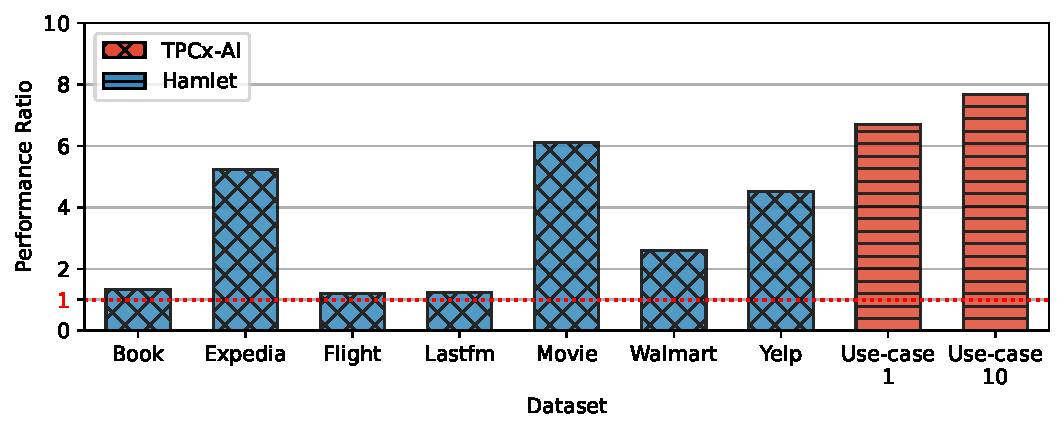
\includegraphics[width=0.7\linewidth]{chapters/05_cost_estimation/figures/real_datasets_speedup.pdf}
    \vspace*{-5mm}
    \caption[Performance gain with factorization on real datasets]{Average Performance ratio of ML models for positive cases ($\text{Time}_M > \text{Time}_F$), split per tested real dataset.}
    \label{fig:5-real-perf-ratio}
\end{figure}

The goal of factorized ML is reducing the number of redundant operations performed during training of a model, to make this process more efficient, i.e., faster. We show the performance gain of factorization over materialization, on real datasets, in \autoref{fig:5-real-perf-ratio}. This shows that exploring factorization is beneficial, as for those cases where it is faster (which is $18\%$ of the tested cases on real datasets), the average speedup is $5.1\times$. In the most extreme cases the training time is reduced by more than $20$ seconds, a reduction by a factor of $27$. In scenarios where training occurs often, e.g., during hyperparameter optimization or online learning this can lead to significant time savings.

% We group the Data and Model characteristics as they both influence the actual computations being executed. The hardware characteristics influence how these computations are carried out on the hardware and are discussed separately. 

\subsection{Data \& Model Characteristics}
\begin{figure}[ht]
    \centering
    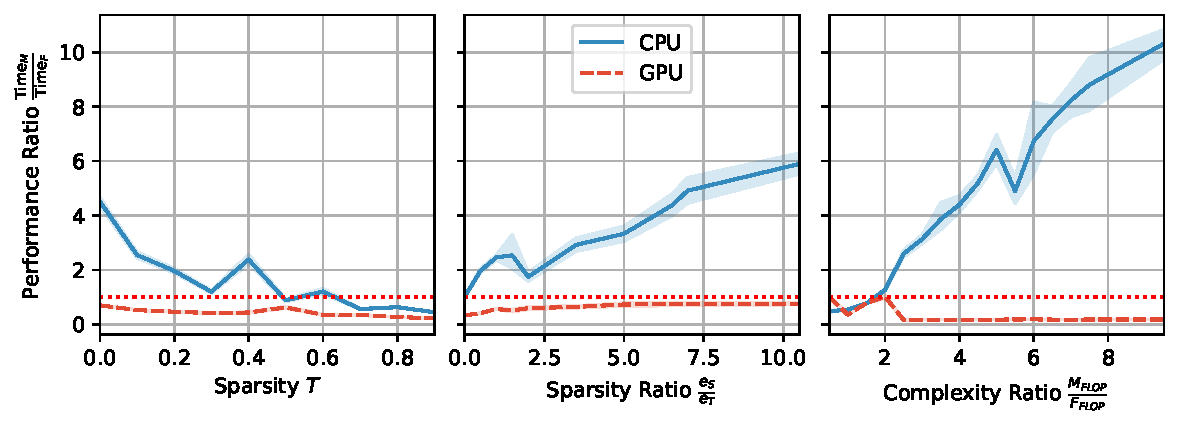
\includegraphics[width=\linewidth]{chapters/05_cost_estimation/figures/motivation_perf_ratio_vs_data_chars.pdf}
    \caption[Performance ratio for various data characteristics]{Performance ratio against various data characteristics. Broken down by compute type (CPU/GPU) and operator type (ML models in the first row \& regular operators in the second). $99\%$ confidence interval shown as shaded area. The sparsity ratio is defined as the sparsity of the source tables $S_k, k\in[1,n]$ divided by the sparsity of target table $T$. Sparsity of $S$ is defined as the total non-zero values in the base tables divided by the total number of cells in the base tables, $\frac{\sum_{k=1}^{n} nnz(S_k)}{\sum_{k=1}^{n} r_{S_k} \times c_{S_k}}$. High sparsity ratio means the target table is relatively sparser than the source tables.}
    \label{fig:5-complexity-ratio-vs-data-chars}
\end{figure}
We show the impact of various data characteristics on the performance ratio in \autoref{fig:5-complexity-ratio-vs-data-chars}. The figure shows a slight negative correlation between performance ratio and sparsity of target table $T$. The second column shows more insight into the relation between performance and sparsity. It shows that when the sparsity ratio is low, i.e., compared to the base tables $S_k$, $T$ has more zero values, factorization is likely slower than materialization. The right-most plots show that a higher complexity ratio ($\frac{M_{FLOPs}}{F_{FLOPS}}$) is likely to lead to factorization being the preferred training method. This is in line with the intuition that factorization is beneficial when it saves redundant computations.

Important to note is that the correlation between these data characteristics and the speedup factorization brings is not as clear when we use GPUs for computation. This is likely due to the fact that the computations are not compute-bound but memory-bound. This view is discussed thoroughly in \autoref{sec:5-gpu-performance-analysis}, where the metrics collected in the profiling experiments are analysed.


\subsection{Hardware Characteristics}
\begin{figure}[ht]
    \centering
    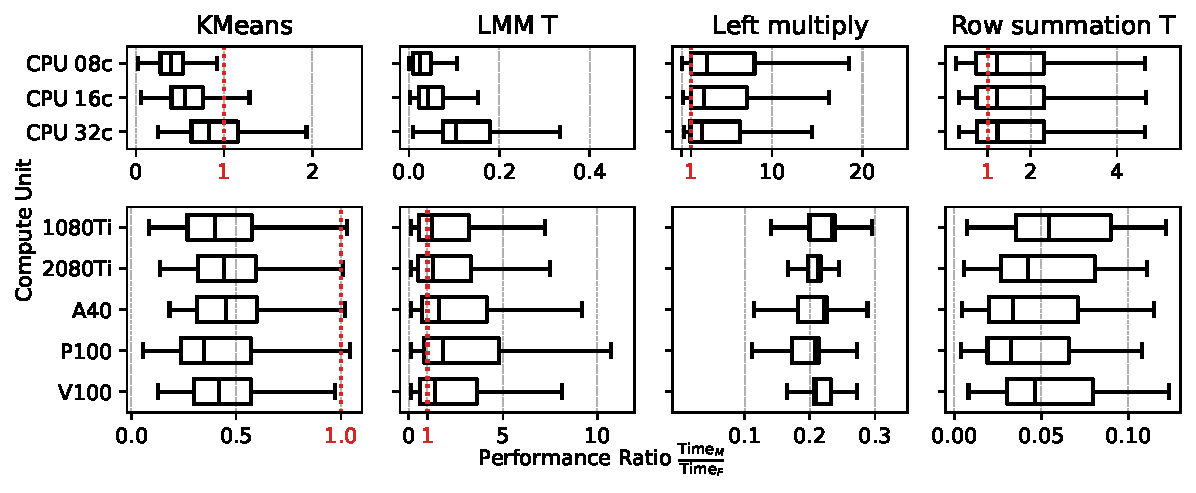
\includegraphics[width=\linewidth]{chapters/05_cost_estimation/figures/motivation_speedup_per_operator_per_gpu.pdf}
    \caption[Performance ratio plotted against hardware]{Performance ratio, of various operators on synthetic data, against hardware. The performance ratio is shown to be affected by hardware choice.}
    \label{fig:5-gpu-characteristics}
\end{figure}
The hardware used for computation impacts the runtime of a program, but here we show it also impacts the F/M trade-off. Different compute unites (i.e., CPU or GPU type) have a different decision boundary for when to use factorization over materialization. This is shown in \autoref{fig:5-gpu-characteristics}. Differing hardware impacts the performance ratio differently per operator. For example, the (mean$\pm$std.) performance ratio of transposed Left Matrix Multiplication on the P100 is $3.03\pm2.70$, while on the V100 it is slightly lower with $2.32\pm2.21$. But, for Left (scalar) multiplication the V100 has the higher performance ratio of $0.21\pm0.04$, against the P100's lower $0.19\pm0.05$.

\begin{table}[ht]
    \centering
    % LTeX: enabled=false
\begin{tabular}{lrrrr}
\toprule
Compute Unit & Mean & Std. Dev. & Count & \% with Speedup \\
\midrule\midrule
CPU 08c & 1.27 & 0.25 & 172 & 1.78\% \\
CPU 16c & 1.32 & 0.34 & 579 & 5.99\% \\
CPU 32c & 1.48 & 0.46 & 2873 & 29.74\% \\
1080Ti & 2.27 & 1.60 & 432 & 4.47\% \\
2080Ti & 1.87 & 1.09 & 425 & 4.40\% \\
A40 & 2.00 & 1.20 & 392 & 4.06\% \\
P100 & 2.52 & 1.84 & 461 & 4.77\% \\
V100 & 1.95 & 1.13 & 404 & 4.18\% \\
\bottomrule
\end{tabular}

    \caption[Performance ratio of ML models for cases where factorization has positive impact.]{Mean performance ratio of ML models for cases where factorization is preferred over Materialization (speedup > 1). This shows hardware choice is a large factor in when to choose factorization over Materialization.}
    \label{tab:5-speedup-per-gpu}
\end{table}

For cases where factorization is preferred over materialization ($\text{Time}_F < \text{Time}_M$), there are large differences between the GPUs. Both the mean performance ratio, and the count of cases where F is faster than M varies greatly, as shown in \autoref{tab:5-speedup-per-gpu}. This shows that the choice of hardware is a large factor in when to choose factorization over materialization.

Another interesting observation can be seen when comparing the performance ratio against the complexity ratio \cite{schijndel_cost_estimation}, for different hardware settings. As explained in \autoref{sec:3-cost-estimation-for-factorized-ml} the complexity is defined as the number of FLOPs needed to perform an operation. The ratio is defined as the complexity of the factorized case divided by the complexity of the materialized case. Thus, per \cite{schijndel_cost_estimation}, the higher this ratio the more beneficial it is to use factorization. However, our experiments show that while this is the case for a lot of operators on CPU, when performing the computations on GPUs this is not always the case. This is shown in \autoref{fig:5-complexity-ratio-vs-performance-ratio}. The next section explores why this is the case.

\begin{figure}[ht]
    \centering
    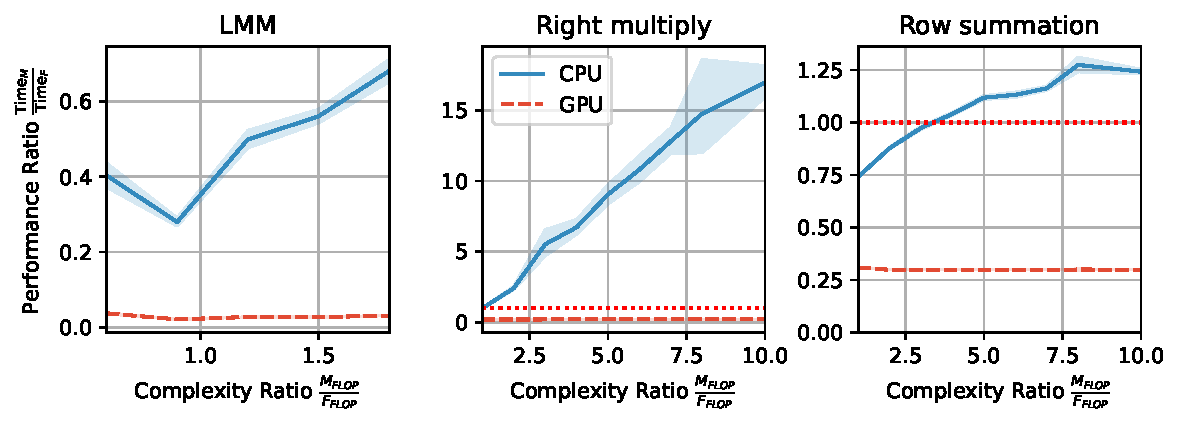
\includegraphics[width=\linewidth]{chapters/05_cost_estimation/figures/motivation_speedup_complexity_ratio.pdf}
    \caption[Performance ratio plotted against complexity ratio]{Performance ratio, of various operators on synthetic data, against complexity ratio, broken down by CPU and GPU. 95\% Confidence interval shown as shaded area. Where a lot of operators show clear correlation between the complexity ratio and the performance ratio on CPU, this is not the case for GPU.}
    \label{fig:5-complexity-ratio-vs-performance-ratio}
\end{figure}


\section{GPU Performance Analysis}
\label{sec:5-gpu-performance-analysis}
A preliminary step for creating an accurate cost model is to understand the performance characteristics of the hardware. This section analyses the profiling metrics collected during the experiments, to understand how the choice of hardware impacts the trade-off between factorization and materialization. A first simple analysis is to compare the memory cost and math cost of the profiled scenarios. Per NVIDIA, a fitting way to estimate the runtime of a GPU program is to compute $max(T_{mem}, T_{math})$. In this formula $T_{mem}$ is the time it takes to transfer data to and from GPU memory, and $T_{math}$ is the time it takes to perform the actual computations. This is in line with the fact that the memory throughput of a GPU is much higher than that of a CPU, and thus the computations are often memory-bound. In this section we show whether this is the case for our experiments, and how we can use this to estimate the runtime of an ML training scenario.

\begin{figure}[ht]
    \centering
    \begin{minipage}{0.50\textwidth}
        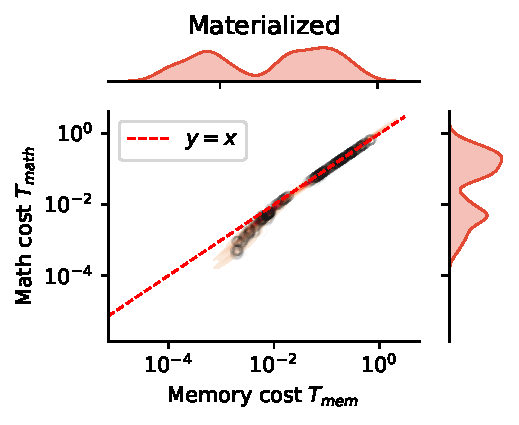
\includegraphics[width=\linewidth]{chapters/05_cost_estimation/figures/profiling-mem-vs-compute-materialized.pdf}
    \end{minipage}\hfill
    \begin{minipage}{0.50\textwidth}
        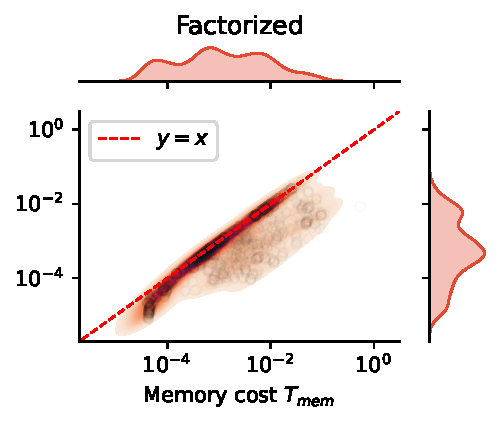
\includegraphics[width=\linewidth]{chapters/05_cost_estimation/figures/profiling-mem-vs-compute-factorized.pdf}
    \end{minipage}
    \caption[Memory cost vs math cost of profiled scenarios]{Memory cost ($T_{mem}$) vs compute cost ($T_{math}$) of profiled scenarios. The memory cost is computed as the total number of bytes read and written to memory divided by the measured average memory bandwidth. The math cost is the number of cycles the Streaming Multiprocessors were active divided by the measured average SM frequency.}
    \label{fig:5-profiling-mem-vs-compute}
\end{figure}

\autoref{fig:5-profiling-mem-vs-compute} shows the distribution of $T_{mem}$ vs $T_{math}$. As expected, these values are highly correlated ($\rho = 0.99$). Almost none of the profiled scenarios have a higher math cost than memory cost, all points are below the $y=x$ line. This shows that the computations are memory-bound, and that the memory cost is a good estimator for the runtime of a scenario. However, the difference between factorization and materialization is substantial. This first becomes obvious when calculating the correlation, for the materialized cases $\rho \text{is} 0.99$, for the factorized cases this is only $0.40$. The cause for this is that with the materialized case the GPU only has to handle a single matrix (or two matrices in the case of matrix multiplication). The normalized matrix used for the factorized case consists of more separate matrices ($S,I,M$), each used in different computations. On average, this reduces both the memory and compute cost. However, it also causes a shift away from the $T_{mem} = T_{math}$ line, as the computations on the different matrices are executed in sequence on the GPU.

\begin{figure}
    \centering
    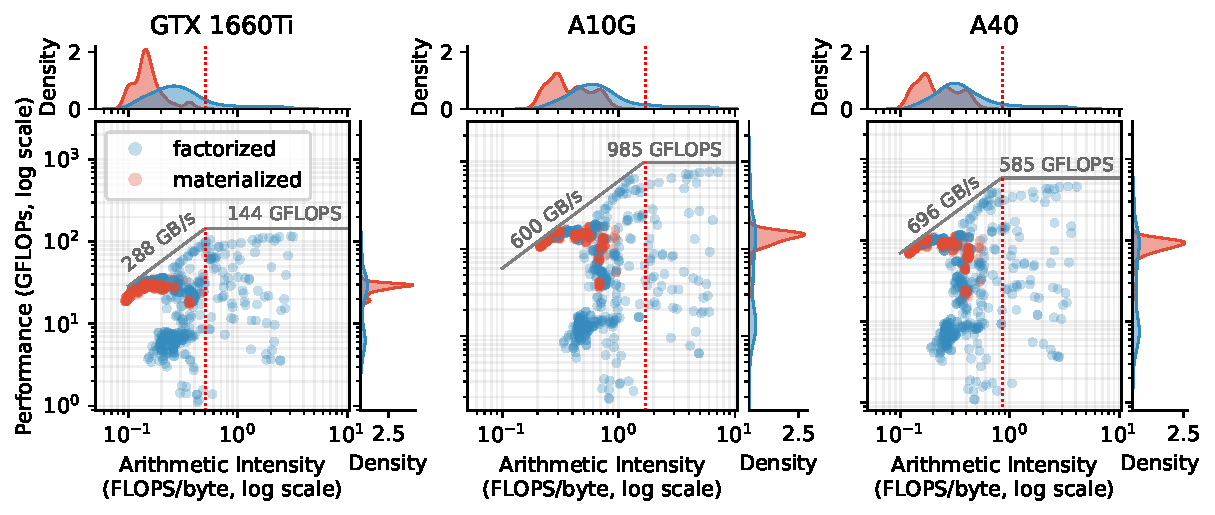
\includegraphics[width=\linewidth]{chapters/05_cost_estimation/figures/roofline-plot.pdf}
    \caption[Roofline chart comparing F/M, per GPU]{Roofline chart showing where the performance of the GPUs lies in the memory-bound vs compute-bound spectrum. The subplots on top and right side of each figure show the distribution along the performance (GFLOPs) and operational intensity (FLOPs/Byte) axes. Similar GPU types have similar distributions. \todo{Write smth about F vs M.}}
    \label{fig:5-roofline-plot}
\end{figure}

\subsubsection*{Roofline Model}
Not only the split in metrics between F and M is interesting, but the difference in efficiency between different GPUs is also substantial. A roofline model can be used to create a visualization for this. It is a “model that offers insight insights \ldots on improving parallel software and hardware for floating point computations” \cite{roofline}. The roofline model shows whether an operator on a given scenario is memory- or compute-bound. The x-axis shows arithmetic intensity of a program in FLOPs per byte (in our case a program is an operator executed on a given dataset), the y-axis the (attainable) performance in GFLOPs. The roofline (top line in grey) shows the bound on performance of a given GPU. It is constructed by taking the maximum memory bandwidth and the maximum number of FLOPs the GPU can perform per second. The point where they meet (\textit{ridge point}) tells you the minimum arithmetic intensity needed to fully utilize a GPUs compute capacities. By plotting programs on such a roofline chart one can reason about whether it is compute- or memory-bound by whether it is to the left (memory bound) or to the right of the \textit{ridge point's} x coordinate (compute bound). This is insightful because it shows where the opportunity for optimization lies by identifying bottlenecks.

The roofline charts for the performed profiling experiments are shown in \autoref{fig:5-roofline-plot}. These charts confirm that almost all scenarios are memory-bound. But, the interesting observation from this plot is the impact of GPU type, and the difference between factorization and materialization. The differences between GPUs are most obvious in the right distribution plots. The A10G and A40 are much more powerful GPUs. On the GTX1660Ti most scenarios reach a low compute performance as they hit the memory bound. The A10G and A40, however, have a much higher memory bandwidth. Thus, the scenarios have reach a higher average performance. The gap these plots show between factorization and materialization gives more valuable insights. The materialized operators have lower arithmetic complexity than their factorized equivalents (shown in top density plots). This means that, on average, the factorized operators are less memory-bound, and thus can utilize a larger part of the GPUs compute capacity. However, the factorized operators show a much larger variance in attained performance (right density plots) due to the fact that the operations on different parts of the normalized matrix are not parallelized. These operators can likely be tweaked, so they can take advantage of the GPUs compute capacity more efficiently.

\todo{Show roofline per operator}

\todo{Add this section showing things like ops:bytes ratio differences between GPUs \& operators?
    % results/full_1/analytical_model/analytical.ipynb}
    \begin{enumerate}
        \item Something like figure 10 in \cite{tvm}. \textbf{Roofline chart.}
        \item Show that \\ \texttt{(dram\_bytes\_read\_sum + dram\_bytes\_write\_sum) / memory\_throughput\_byte\_weighted\_mean} is a good estimator for duration.
    \end{enumerate}
}

\section{Feature Engineering}
\label{sec:5-feature-engineering}
\todo{
    Data Preprocessing steps
    \begin{enumerate}
        \item Collection of data characteristics
        \item Complexity
        \item ratios: complexity, sparsity
        \item Memory costs from profiling metrics
        \item Computation costs from profiling metrics
    \end{enumerate}
    Finally show schema of the final dataset used for training the models.
}

$T_{mem} = \frac{dram\_bytes\_read\_sum + dram\_bytes\_write\_sum}{memory\_throughput\_byte\_weighted\_mean}$
$T_{math} = \frac{sm\_active\_cycles\_sum}{sm\_frequency\_weighted\_mean}$



\begin{figure}[ht]
    \centering
    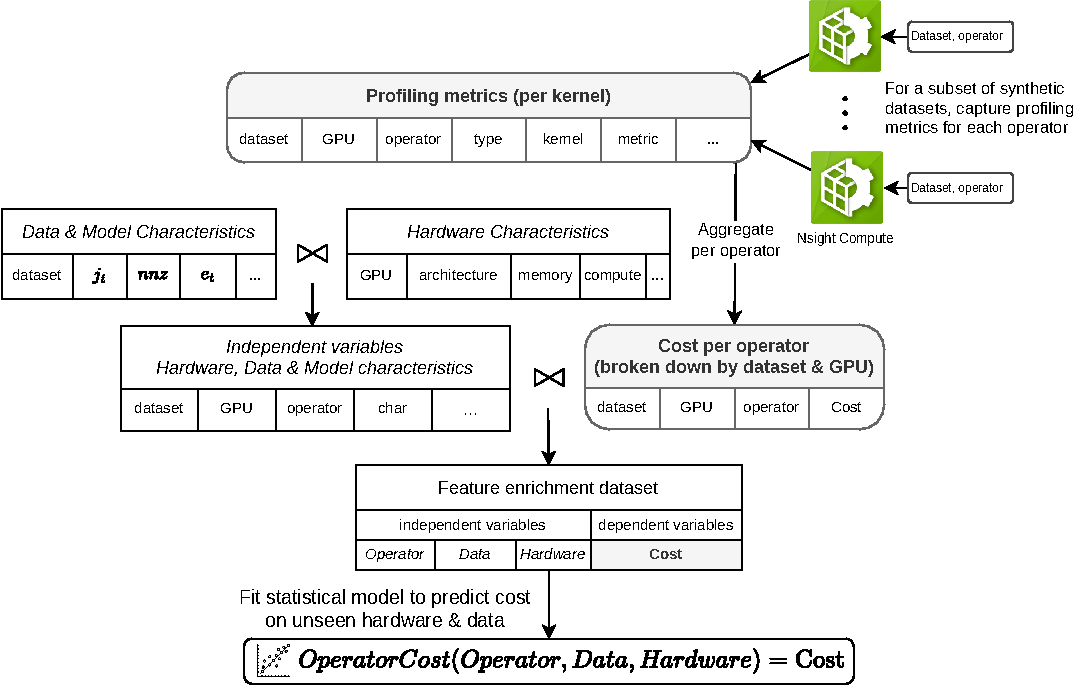
\includegraphics[width=\linewidth]{chapters/05_cost_estimation/figures/feature-engineering.pdf}
    \caption[Feature enrichment workflow]{Workflow of enriching the collected data with additional features from the profiling experiments. Items related to these profiling experiments are \textbf{bolded}, while the features from the data, model \& hardware characteristics are \textit{italicized}.}
    \label{fig:5-feature-enrichment}
\end{figure}

\section{Cost Models}
\label{sec:5-cost-models}
\todo{Detail the full process going from data to Cost model, what features where used, and what is the inner architecture?\\Show each of the factors is significant. Data, Hardware, Model parameters.\\Show R2 score to compare between models.}



\subsection{Analytical}
\begin{figure}[ht]
    \centering
    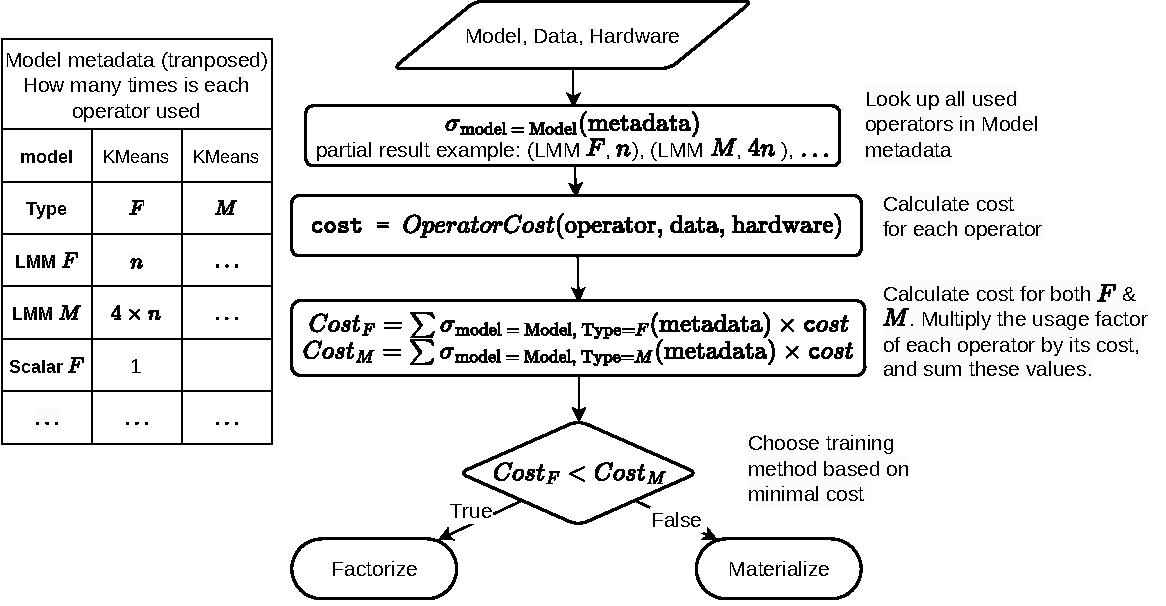
\includegraphics[width=\linewidth]{chapters/05_cost_estimation/figures/analytical-architecture.pdf}
    \caption[Analytical Estimator Architecture]{Architecture of the Analytical Estimator. Shows the control flow of inputs to a final decision on whether to use factorization or materialization. $OperatorCost$ is the function as defined in \autoref{fig:5-feature-enrichment}.}
    \label{fig:5-analytical-architecture}
\end{figure}

\subsection{Statistical}
The goal for this statistical estimator is to still be explainable, while providing higher performance than the hand tuned decision rules from related works. We use a variety of models, which all use Linear Regression at their core. We start with a singular regressor, and, by fine-tuning, end up at more complex models, with ensembles of linear regression models. The architecture of each of the statistical models is explained in \autoref{fig:5-statistical-architecture}.


\todo{
    \begin{enumerate}
        \item Linear Regression
        \item Difference with Analytical: predict time\_saved instead of runtime for both F and M.
              % \item For each fitted regressor we use Recursive feature elimination with cross-validation to select features \cite{rfecv}.
        \item Start with the simplest single linear regression model, continue to ensembles.
    \end{enumerate}
}

\begin{figure}[ht]
    \centering
    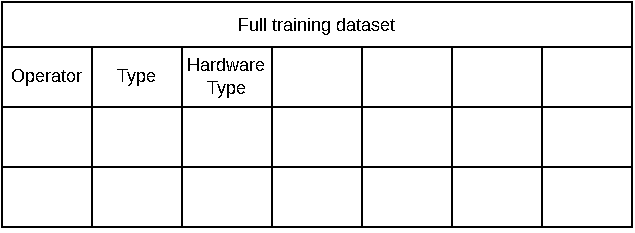
\includegraphics[width=\linewidth]{chapters/05_cost_estimation/figures/statistical-architecture.pdf}
    \caption[Statistical Estimator Architecture]{Architecture of the Statistical Estimators. Shows how the data, and estimators, are split for each model. The final split-level belonging to each respective model is coloured in the same colour. For STAT.5 we show the linear regression ensemble fit to the data. For clarity, we leave this out for the other models. Each box represents a regression model, the same-coloured boxes, connected via dotted lines, are combined into an ensemble to end up with the statistical cost estimators.}
    \label{fig:5-statistical-architecture}
\end{figure}

\subsubsection*{STAT.1 Linear Regressor Fit to Full Training Set}
The first linear regressor is trained on the full training set, which includes all operators. The rationale behind this approach is that there is likely a relationship between the performance of individual operators and the performance of the models in which they are used. By training the regressor on the full set of operators, we aim to capture these relationships and use them to improve the accuracy. This model predicts the time saved by choosing factorization over materialization.

\subsubsection*{STAT.2 Linear Regressor Fit to Model Runtimes}
The second linear regressor is trained on the runtimes of the models. With this model we find whether including the operators adds utility. Like STAT.1, this model predicts the time saved by choosing factorization over materialization.

\subsubsection*{STAT.3 Separate Regressors for F and M}
This model is an ensemble of two linear regressors, one for factorization and one for materialization. By training separate regressors for factorization and materialization, we aim to capture the relationships between independent variables and runtime more explicitly than is done by the previous models. Each internal regressor predicts the runtime of the scenario under test, and the final prediction is which is predicted to be faster.

\subsubsection*{STAT.4 Separate Regressors for each Model Type}
Much like STAT.3 this estimator is also a combination of multiple inner regressors. However, instead of having one regressor for each factorization and materialization, we have one regressor for each model type. This is done to capture the differences in the relationships between independent variables and runtime for different model types. Like the first two models, this model predicts the time saved by choosing factorization over materialization (by predicting whether time is saved by choosing F).

\subsubsection*{STAT.5 Separate Regressors CPU and GPU}
In previous sections we have shown that the choice of hardware plays a large factor in the trade-off we are researching, therefore it is likely there are differences in the relationships between independent variables and runtime between CPU and GPU. A single linear regression model is likely unable to capture these differences. Therefore, we test the performance of a couple of estimators, one which is only fit to CPU scenario's, and one which is only fit to GPU scenario's.

\subsubsection*{STAT.6 Separate Regressors for F, M and Model Type}
The last version of the statistical model we created is a combination of STAT.4 and STAT.3. By training separate regressors for every combination of factorization, materialization and model type, we allow the models to capture differences between the groups more freely.

\subsubsection*{STAT.7 Separate Regressors Each Dimension}
The last, most granular, ensemble is one that has a separate regressor for each combination of factorization, materialization, model type and hardware. This is done to capture the differences in the relationships between independent variables and runtime for each combination of the dimensions.


\subsubsection{Statistical Model Evaluation}
\todo{Text to go with \autoref{fig:5-statistical-model-evaluation}.}

\begin{figure}[ht]
    \centering
    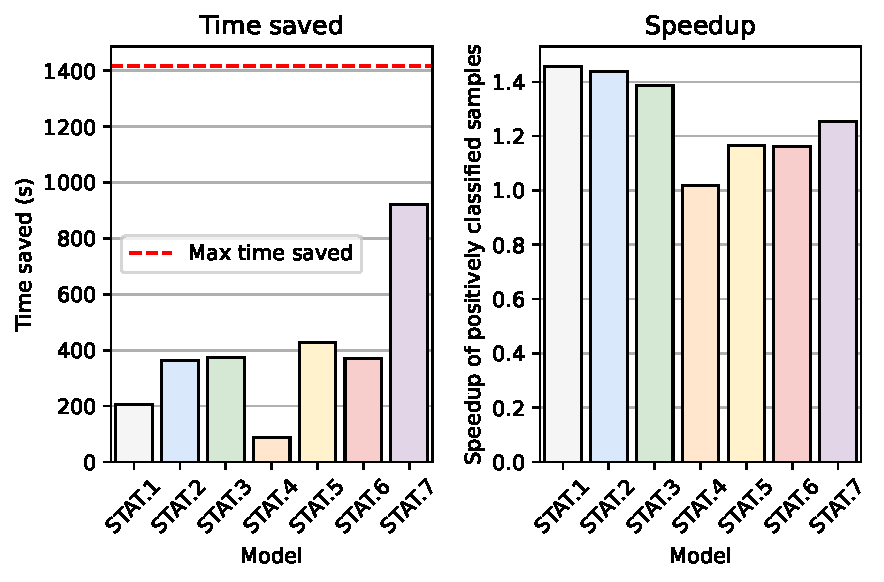
\includegraphics[width=\linewidth]{chapters/05_cost_estimation/figures/stat-models-compare.pdf}
    \caption[Statistical Model Evaluation]{Evaluation of the statistical models on the test set (synthetic data, only models). The first two plots show statistics of those scenarios where the estimator predicts factorization to be faster. The last plot shows the time saved, as a fraction of the total to-be-saved time (by a perfect estimator), when using this estimator.}
    \label{fig:5-statistical-model-evaluation}
\end{figure}

\subsection{Deep Learning}
\todo{Write, show architecture, show results. Use \cite{TreeRNN}, as it shows good performance in \cite{tvm}.}

\subsection{Hybrid}

\subsection{Meta-results}
\todo{Inference speed, training time.}

% !TEX root = ../../main.tex

\chapter{Evaluation}
\label{chapter:evaluation-discussion}
This chapter shows Contribution \textbf{C.2}: A robust cost estimator for Amalur's factorized ML framework, and a comparison with the state-of-the-art in \autoref{sec:eval-model-evaluation}. Before that, we show how results were collected in \autoref{sec:6experiment-setup}. The \hyperref[sec:eval-discussion]{third section} of this chapter provides an in-depth interpretation of the results as well as a critical view on the implications and limitations of this work.

\section{Experiment Setup}
\label{sec:6experiment-setup}

This section goes into detail about anything needed to replicate the results. This includes the experimental environment (\hyperref[subsec:6-software]{Software}, \hyperref[subsec:6-datasets]{Datasets} \& \hyperref[subsec:6-hardware]{Hardware}),  and how the data was treated to ensure sound results for the cost estimators (\hyperref[subsec:6-validation-strategy]{validation strategy}). For further details and implementations please refer to the GitHub repository\footnote{\todo{TODO}}.

\subsection{Software}
\label{subsec:6-software}
The factorized ML framework (Amalur \cite{amalur}) is implemented in Python (3.10.4) and uses SciPy (1.8.0), NumPy (1.22.4) and CuPy (12.1.1). All experiments where ran in a Docker container with an image based on Nvidia's base image with CUDA 12.1.1 and Ubuntu 20.04\footnote{\href{https://hub.docker.com/layers/nvidia/cuda/12.1.1-devel-ubuntu20.04/images/sha256-5bd13c67a4479a1c13238b470d89a92937ce68ba5f21b930d50c463e3314f657?context=explore}{nvidia/cuda:12.1.1-devel-ubuntu20.04}}.

The choice to use CuPy as the backend for the factorized ML framework was made to ensure that the experiments could be run on both CPU and GPU. CuPy is a GPU-accelerated library for numerical computations that is compatible with NumPy and SciPy \cite{cupy_learningsys2017}. This allows for minimal changes to the codebase whether you are using GPU or CPU. To allow for exploitation of multiple cores for sparse matrix multiplication\footnote{\url{https://github.com/flatironinstitute/sparse_dot}} we use MKL (Intel Math Kernel Library) \cite{intel-mkl} as NumPy's backend for the CPU experiments.

For collecting the GPU metrics we use NVIDIA's Nsight Compute (ncu)\footnote{\url{https://docs.nvidia.com/nsight-compute/NsightComputeCli/index.html}} which is a command-line profiler that collects detailed performance metrics from the GPU. The metrics are collected in a CSV file for downstream analysis, detailed in \autoref{sec:5-feature-engineering}.

\subsection{Datasets}
\label{subsec:6-datasets}
The datasets used in the experiments are a mix of synthetic and real-world datasets. The synthetic datasets are used to generate a training set to train the cost estimators on. The real-world datasets are used to validate the cost estimators on unseen data.

\subsubsection{Synthetic Datasets}
To create the synthetic datasets with a wide variety of data characteristics the data generator from \cite{schijndel_cost_estimation} was used, which in turn is an adaptation of the data generator\footnote{\url{https://github.com/delftdata/valentine-data-fabricator}} from \cite{valentine-data-generator}.

In total, we generated $2415$ datasets, each being a two-table join. All other parameters were varied, the values are shown in \autoref{tab:6-synthetic-dataset-characteristics}.

\todo{Expand this! Explain star schema (and show example)?}

\begin{table}[ht]
  \centering
  \begin{tabular}{llr}
    \toprule
    Data Characteristic             & Symbol    & Range                              \\ \midrule \midrule
    Target Sparsity                 & $e_T$     & $[ 0.0\text{,\ \ } 0.9]$           \\
    $S_1$ (Entity) table rows       & $r_{S_1}$ & $[ 40,000\text{,\ \ } 1,000,000]$  \\
    $S_1$ (Attribute) table rows    & $r_{S_2}$ & $[ 526\text{,\ \ } 1,000,000]$     \\
    $S_1$ (Entity) table columns    & $c_{S_1}$ & $[ 1\text{,\ \ } 50]$              \\
    $S_1$ (Attribute) table columns & $c_{S_2}$ & $[ 2\text{,\ \ } 50]$              \\
    Target table rows               & $r_T$     & $[ 60,000 \text{,\ \ } 1,000,000]$ \\
    Target table columns            & $c_T$     & $[ 11\text{,\ \ } 100]$            \\
    Tuple ratio                     & $\rho$    & $[ 1\text{,\ \ } 190]$             \\
    Feature ratio                   & $\tau$    & $[ 0.2\text{,\ \ } 1]$             \\
    Join Type                       & $j_T$     & Inner, left or outer.              \\
    Selectivity                     & $\sigma$  & $[ 1.0\text{,\ \ } 2.0]$           \\
    \bottomrule
  \end{tabular}
  \caption{Ranges of data characteristics for the generated synthetic datasets}
  \label{tab:6-synthetic-dataset-characteristics}
\end{table}


\subsubsection{Real-world Datasets}
The synthetic datasets are convenient for testing and training purposes. However, to assess whether the cost estimators are generalizable to real-world data, we use real-world datasets for validation.

\paragraph{Project Hamlet \cite{2016-hamlet-sigmod}}
The Hamlet datasets are widely used in related literature \cite{2016-hamlet-sigmod, amalur, morpheus,orion_learning_gen_lin_models}. The Hamlet datasets are a set 7 datasets specifically designed to mimic data integration scenarios is an ML workflow. The original datasets where created to evaluate inner join scenario's. As we are also interested in other join types, some rows were removed from different source tables for these join types. The data characteristics of these datasets are shown in \autoref{tab:6-hamlet-characteristics}.


\begin{table}[ht]
  \centering
  \begin{tabular}{p{0.12\linewidth}rrrrrrr}
    \toprule
    Dataset$\rightarrow$ Characteristic $\downarrow$ & Book  & Expedia & Flight & Lastfm & Movie & Walmart & Yelp  \\
    \midrule \midrule
    $r_T$                                            & 253K  & 942K    & 66.5K  & 344K   & 1M    & 422K    & 216K  \\
    $c_T$                                            & 81.7K & 52.3K   & 13.7K  & 55.3K  & 13.3K & 2.44K   & 55.6K \\
    $n$                                              & 2     & 3       & 4      & 2      & 2     & 3       & 2     \\
    $r_{S_1}$                                        & 27.9K & 942K    & 66.5K  & 5K     & 6.04K & 422K    & 11.5K \\
    $r_{S_2}$                                        & 50K   & 11.9K   & 540    & 50K    & 3.71K & 2.34K   & 43.9K \\
    $r_{S_3}$                                        &       & 37K     & 3.17K  &        &       & 45      &       \\
    $r_{S_4}$                                        &       &         & 3.17K  &        &       &         &       \\
    $c_{S_1}$                                        & 28K   & 27      & 20     & 5.02K  & 9.51K & 1       & 11.7K \\
    $c_{S_2}$                                        & 53.6K & 12K     & 718    & 50.2K  & 3.84K & 2.39K   & 43.9K \\
    $c_{S_3}$                                        &       & 40.2K   & 6.46K  &        &       & 53      &       \\
    $c_{S_4}$                                        &       &         & 6.47K  &        &       &         &       \\
    \bottomrule
  \end{tabular}
  \caption[Hamlet dataset characteristics]{Hamlet dataset characteristics. $r$ is the number of rows, $c$ is the number of columns, and $n$ is the number of tables. The subscripts denote which table the characteristic belongs to. }
  \label{tab:6-hamlet-characteristics}
\end{table}


\paragraph{TPCx-AI \cite{tpcx-ai}} We also evaluate on a scenario even more realistic than Hamlet, as it is based on a real-world benchmark used to evaluate end-to-end ML platforms. As that is not the focus of this work, we use only two out of the ten use cases, namely the first and the tenth use case. This benchmark also provides a data generator with scalable generation capabilities, through setting different scale factors from $0.01-0.5$ we generated $18$ datasets for each use case. The data characteristics of the resulting datasets can be found in \autoref{fig:tpcx-ai-data-chars}.
\begin{figure}
  \centering
  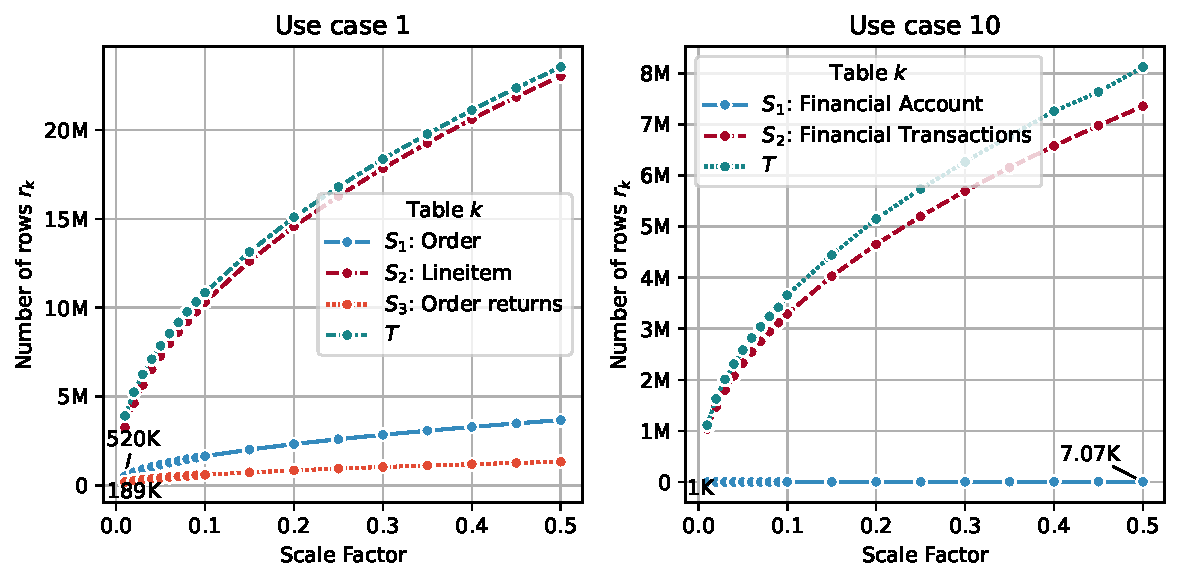
\includegraphics[width=\linewidth]{chapters/06_evaluation/figures/tpcx-ai-data-chars.pdf}
  \caption[TPCx-AI dataset sizes for used scale factors.]{TPCx-AI dataset sizes for used scale factors. The number of columns is independent of the scale factors. For use case 1: $c_1=3, c_2=4, c_3=3, c_T=7$. For use case 10: $c_1=2, c_2=7, c_T=5$.}
  \label{fig:tpcx-ai-data-chars}
\end{figure}

\todo{Explain use cases.}



\subsection{Hardware}
\label{subsec:6-hardware}

The experiments are run on a relatively large set of different machines because of the need to test on varying hardware. Most experiments were run on the Delft AI Cluster\footnote{\url{https://daic.tudelft.nl/}} which made it possible to run experiments on different GPU architectures. Because profiling was not possible on this cluster, some profiling experiments were run on a local machine, AWS, and resources of the Web Information Systems group\footnote{\url{https://www.wis.ewi.tudelft.nl/}}. The exact overview of which experiment was run on which machines is shown in \autoref{tab:6-hardware-overview}.

\begin{table}[ht]
  \centering
  % LTeX: enabled=false
\begin{tabular}{p{0.15\linewidth}p{0.19\linewidth}p{0.10\linewidth}p{0.20\linewidth}l}
    \toprule
    Experiment type                                                 & Machine                                                         & \hspace{0pt}Architecture                                  & Compute Unit           & Experiment       \\
    \midrule\midrule
    \multirow[t]{3}{*}{\parbox{1\linewidth}{\vspace{1.5cm}profile}} & WIS ST4                                                         & Ampere                                                    & GPU A40                & \texttt{GPU-P-1} \\
    \cline{2-5}
                                                                    & AWS G5.xlarge                                                   & Ampere                                                    & GPU A10G               & \texttt{GPU-P-2} \\
    \cline{2-5}
                                                                    & Personal Workstation                                            & Turing                                                    & GPU 1660Ti             & \texttt{GPU-P-3} \\
    \cline{1-5}
    \multirow[t]{8}{*}{\parbox{1\linewidth}{\vspace{4cm}runtime}}   & \multirow[t]{5}{*}{\parbox{1\linewidth}{\vspace{2cm}DAIC}}      & Ampere                                                    & GPU A40                & \texttt{GPU-T-1} \\

                                                                    &                                                                 & Volta                                                     & GPU V100               & \texttt{GPU-T-2} \\

                                                                    &                                                                 & Pascal                                                    & GPU P100               & \texttt{GPU-T-3} \\

                                                                    &                                                                 & Turing                                                    & GPU 2080Ti             & \texttt{GPU-T-4} \\

                                                                    &                                                                 & Pascal                                                    & GPU 1080Ti             & \texttt{GPU-T-5} \\
    \cline{2-5}
                                                                    & \multirow[t]{3}{*}{\parbox{1\linewidth}{\vspace{2.3cm}WIS ST4}} & \multirow[t]{3}{*}{\parbox{1\linewidth}{\vspace{2.3cm}—}} & EPYC 7H12 CPU 8 cores  & \texttt{CPU-T-1} \\

                                                                    &                                                                 &                                                           & EPYC 7H12 CPU 16 cores & \texttt{CPU-T-2} \\

                                                                    &                                                                 &                                                           & EPYC 7H12 CPU 32 cores & \texttt{CPU-T-3} \\
    \cline{1-5}
    \bottomrule
\end{tabular}

  \caption[Experiment to machine mapping]{Experiment to machine mapping. The experiment type is either profiling or runtime. Profiling experiments are used to collect the hardware specific metrics for our training data. Runtime experiments are used to gather data on the runtime of the factorized ML framework compared to materialized learning.}
  \label{tab:6-hardware-overview}
\end{table}

\subsection{Experiment Setting}
To ensure reliable training data all runtime experiments were run with a repetition count of $30$. The profiling experiments were not repeated, as NCU ensures actionable and deterministic results through, e.g., replaying kernel launches \cite{nsight_compute}. All experiments were run in a containerized environment to ensure reproducibility. The profiling experiments were run with the same image as the runtime experiments, to ensure that the same environment was used for both. Docker\footnote{\url{https://www.docker.com/}} was used as the container runtime, except on the DAIC cluster which enforces the use of Apptainer\footnote{\url{https://apptainer.org/}} image.

\subsection{Validation Strategy}
\label{subsec:6-validation-strategy}

As the possible set of data, model, and hardware characteristics is extremely large, we need to be confident in the ability of our estimator to make accurate predictions for unseen scenarios. To ensure this we use a very strict train-validate-test split. 70\% of the samples from the synthetic datasets are used in the training set. The remaining 30\% is used as a validation set. The real-world datasets are used solely as a test set. As they are not used in the training of the cost estimators they should give an accurate view of the performance in unseen scenarios, whether this is actually the case is shown in \autoref{subsubsec:6-real-datasets}. To guarantee the same robustness in the hardware dimension we use a similar approach, completely keeping the samples of two of the experiments (\texttt{GPU-T-5} \& \texttt{CPU-T-3}\todo{check}) separate for testing. For the last dimension, the model characteristics, we carry out an ablation study (see \autoref{subsubsec:6-ablation}) to see the effect of different models on the performance of the cost estimators.


% \begin{figure}[ht]
%   \centering
%   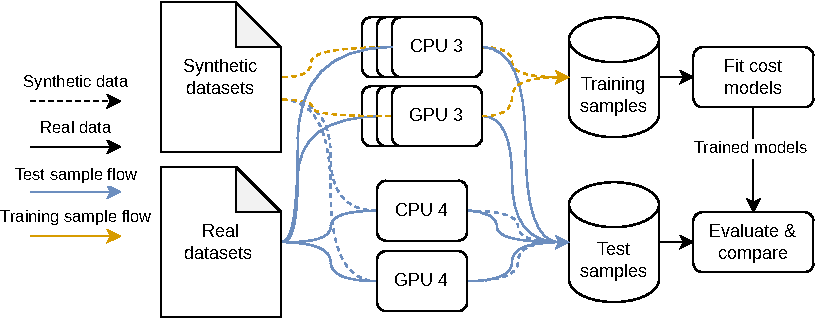
\includegraphics[width=0.8\linewidth]{chapters/06_evaluation/figures/experiment-pipeline.pdf}
%   \caption{\todo{update} Overview of the planned experiments: combinations of datasets and machines we run the experiments
%     on. }
%   \label{fig:enter-label}
% \end{figure}

\section{Cost Model Performance and Comparative Analysis}
\label{sec:eval-model-evaluation}

In this section we answer
\begin{itemize}
  \item[RQ.2] How can we accurately predict the optimal choice between factorized or materialized training of a Machine Learning model, on CPU and GPU, through leveraging knowledge about model, data, and hardware characteristics?
\end{itemize}

We first display that the cost estimator generalizes well to new scenarios. Then we show how the cost estimators compare to the state-of-the-art in cost estimation for Factorized ML training.

\subsection{Exploring Generalizability}
The utility of our strict train-validate-test split is shown here. We show that the cost estimators generalize well to new scenarios.

\subsubsection{Performance with Real Datasets}
\label{subsubsec:6-real-datasets}

\subsubsection{Ablation Study}
\label{subsubsec:6-ablation}


\subsection{Cost Estimator Comparison}


\section{Discussion}
\label{sec:eval-discussion}


% !TEX root = ../../main.tex

\chapter{Conclusion}

\label{chapter:conclusion}
In closing, we consolidate the key contributions and discoveries of this thesis in \autoref{sec:7-contributions}. Additionally, we acknowledge the limitations and outline potential areas for future research in \autoref{sec:7-future-work}.

\section{Cost Estimation for Factorized Machine Learning}
\label{sec:7-contributions}
Our research explores the dynamics of cost estimation for factorized machine learning, emphasizing the comparative performance of GPUs against CPUs. We find that GPU training exhibits distinct cost characteristics from CPU training, which significantly influences cost model design and optimization of factorized machine learning processes.

Previous cost estimation methodologies have predominantly centered on CPU contexts, resulting in inaccuracies when extrapolated to GPU environments. Our analysis reveals a pronounced difference in the speedup of factorized model training between CPU and GPU platforms. This discrepancy stems from the distinct architectural designs and processing capabilities of GPUs, which necessitates a tailored approach to cost estimation.

Through empirical research and extensive experimentation, we have formulated an innovative cost model that is tuned to the nuances of GPU computation. Our model diverges from existing methods by incorporating a deeper understanding of GPU architecture, and by leveraging a more comprehensive set of features to decide the training approach.

By accounting for the unique cost factors associated with GPU usage, we provide a more reliable framework for predicting whether factorization is beneficial. The results of our comparative analysis demonstrate that our cost model outperforms existing methods, both for CPU and GPU scenarios. In the tested scenarios on real-world datasets, for which a perfect model would result in $1667$ seconds saved, the SOTA cost model achieves a time loss of $507$s. Using our hybrid cost model would save $1350$s, reaching almost $80\%$ of the maximum possible utility.

This progress in cost estimation facilitates the broader adoption of factorized machine learning within the industry, enabling considerable time savings in scenarios that use intensive training. Such scenarios include the training of large models, hyperparameter optimization, and real-time training. The impact of using our cost model in the ML workflow is minimal, but when factorization is faster, we achieve an average speedup of $3.8\times$. The largest hurdle for a Data Scientist to use this approach is the adaption of their data integration workflow, so it fits into the factorized ML framework, which currently is a manual process.

Despite promising results, our model comes with certain limitations. The need to account for the unique characteristics of GPU computation introduces complexity into our model, which makes its predictions less explainable than the state-of-the-art models. Another risk associated with the added complexity is overfitting to the current implementation. How our cost model performs when training is done with another implementation of factorized learning is uncertain. Furthermore, the introduction of new machine learning models requires additional work to adapt our cost model accordingly. These challenges highlight areas for future research and improvement. Nevertheless, the benefits of our model in terms of accuracy and efficiency make it a valuable contribution to the field of factorized machine learning.

\section{Future Work}
\label{sec:7-future-work}
As we look forward, there are several promising directions for future work. This thesis has demonstrated the value of factorized machine learning in real-world settings, but to facilitate its adoption in the industry, steps need to be taken. One such step could be the integration of factorized machine learning models into widely used frameworks like TensorFlow and PyTorch. This would not only enhance the practicality and reach of factorized machine learning but also open up opportunities for investigating cost estimation. Given the maturity of these frameworks and the extensive research already conducted to optimize their training processes, this could significantly advance our understanding of cost dynamics in factorized machine learning.

Moreover, this integration could also enable the exploration of factorized machine learning in a distributed setting. This would be a significant advancement, as it would allow us to leverage the power of distributed computing to further enhance the efficiency and scalability of factorized machine learning models. This could potentially lead to breakthroughs in handling larger datasets and more complex computations, thus broadening the scope and impact of factorized machine learning.

In terms of future steps specifically for cost estimation in factorized machine learning, we propose two main areas of focus. Firstly, other types of cost models could be explored, such as those based on micro benchmarking. This involves conducting performance tests on individual operations before running a training scenario. The insights gained from these benchmarks could then be used to make informed decisions between materialization and factorization. This could improve accuracy as the actual datasets can be used for these benchmarks. However, consideration must be given to keeping the overhead of such an approach low. Another direction that could complement our proposed approach is the exploration of online training. This would involve continuously updating the model as new scenarios are tested, leading to a continuously improving model. Such an approach would be particularly valuable in a real-world factorized machine learning framework.

Second, we could expand on the profiling experiments conducted in this thesis. By conducting more extensive profiling experiments, on model training scenarios instead of individual operators, we could gain a deeper understanding of the cost dynamics of factorized machine learning. This would allow us to refine our cost model further and potentially identify new cost factors that could be incorporated into the model. However, this would require a significant investment in time and resources, as profiling experiments are time-consuming and computationally expensive.

Despite the challenges, such as higher complexity and the need for additional work with the introduction of new machine learning models, our model makes a valuable contribution to the field in terms of accuracy and efficiency. These future directions highlight the potential for continued refinement and expansion of our cost model, contributing to the ongoing advancement of factorized machine learning.



%----------------------------------------------------------------------------------------
%	THESIS CONTENT - APPENDICES
%----------------------------------------------------------------------------------------

\appendix % Cue to tell LaTeX that the following "chapters" are Appendices

% Include the appendices of the thesis as separate files from the Appendices folder
% Uncomment the lines as you write the Appendices

\chapter{Detailed datasets}


\section{Real datasets}
\subsection{TPCx-AI}

\begin{figure}[ht]
    \centering
    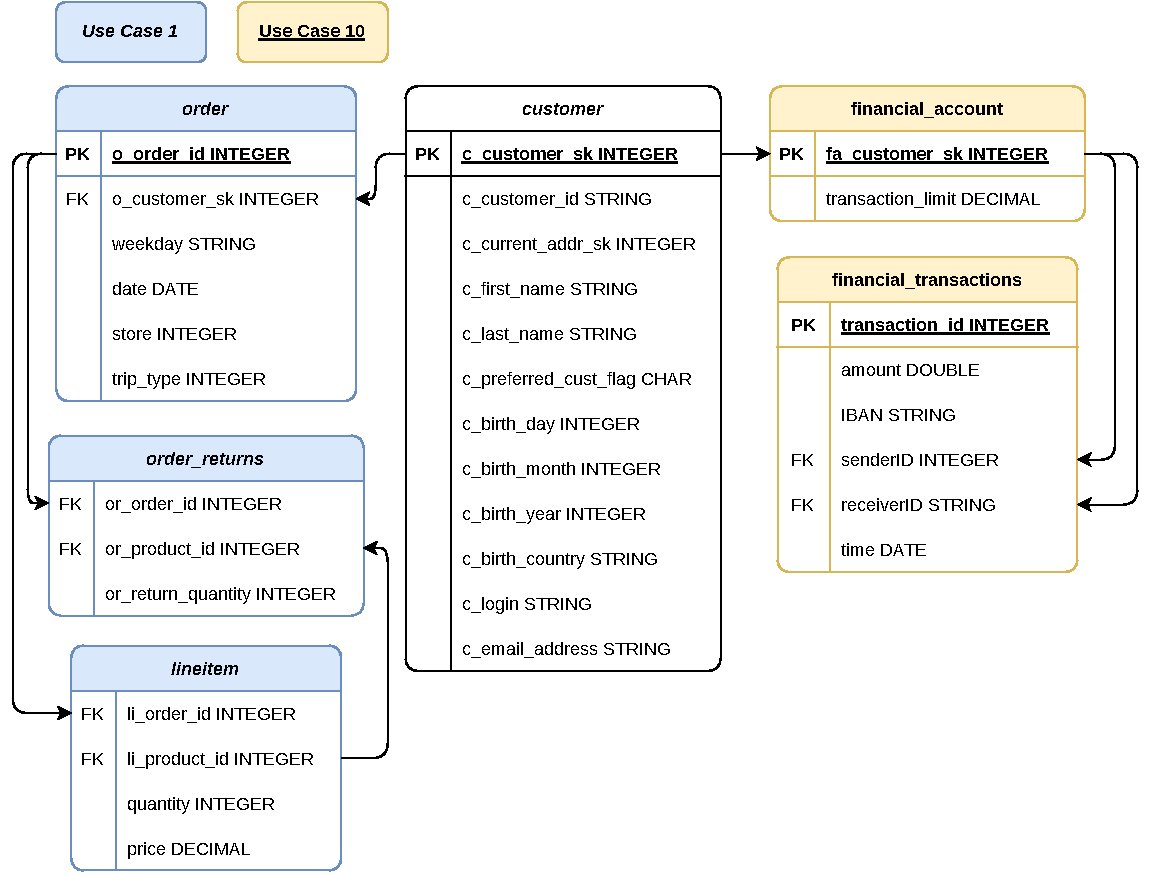
\includegraphics[width=0.99\linewidth]{appendices/figures/tpc-ai-schema.pdf}
    \caption{Simplified schema from the TPCx-AI \cite{tpcx-ai} benchmark. Only schemas used in experiments are shown.}
    \label{fig:appendix-tpc-ai-schema}
\end{figure}
\chapter{GPU Characteristics}
\label{appendix:gpu-characteristics}

\begingroup
\renewcommand{\arraystretch}{1.5}
\begin{table}
    % LTeX: enabled=false
\begin{tabular}{p{0.11\linewidth}p{0.08\linewidth}p{0.12\linewidth}rrrrrrr}
\toprule
 &  GPU $\rightarrow$ & & P100 & 1080Ti & V100 & 2080Ti & 1660Ti & A40 & A10G \\
Group $\downarrow$ & Unit $\downarrow$ & Character-\newline istic$\downarrow$ &  &  &  &  &  &  &  \\
\midrule\midrule
\multirow[t]{3}{\linewidth}{} & \multirow[t]{3}{\linewidth}{} & Architecture & Pas. & Pas. & Vol. & Tur. & Tur. & Amp. & Amp. \\
 &  & Number of SM & 56 & 28 & 80 & 68 & 24 & 84 & 72 \\
 &  & Cores & 3,584 & 3,584 & 5,120 & 4,352 & 1,536 & 10,752 & 9216 \\
\cline{1-10} \cline{2-10}
\multirow[t]{2}{\linewidth}{Cache Size} & KB/SM & L1 & 24 & 48 & 128 & 64 & 64 & 128 & 128 \\
\cline{2-10}
 & MB & L2 & 4.0 & 2.8 & 6.2 & 5.5 & 1.5 & 6.0 & 6 \\
\cline{1-10} \cline{2-10}
\multirow[t]{2}{\linewidth}{Clock Speed} & \multirow[t]{2}{\linewidth}{MHz} & Base & 1,126 & 1,480 & 1,230 & 1,350 & 1,500 & 1,305 & 1320 \\
 &  & Max Boost & 1,303 & 1,582 & 1,370 & 1,545 & 1,770 & 1,740 & 1710 \\
\cline{1-10} \cline{2-10}
\multirow[t]{4}{\linewidth}{Memory} & bit & Bus Width & 4,096 & 352 & 4,096 & 352 & 192 & 384 & 384 \\
\cline{2-10}
 & GB & Size & 16 & 11 & 32 & 11 & 6 & 48 & 24 \\
\cline{2-10}
 & MT/S & Clock & 1,430 & 11,000 & 1,750 & 14,000 & 12,000 & 7,248 & 6,252 \\
\cline{2-10}
 & GB/s & Bandwidth & 732 & 484 & 900 & 616 & 288 & 696 & 600 \\
\cline{1-10} \cline{2-10}
\multirow[t]{3}{\linewidth}{Processing Power} & \multirow[t]{3}{\linewidth}{TFLOPS} & Half Precision & 21.20 & 0.17 & 112.22 & 23.50 & 9.22 & 149.68 & 31.52 \\
 &  & Single Precision & 10.60 & 10.61 & 14.03 & 11.75 & 4.61 & 37.42 & 31.52 \\
 &  & Double Precision & 5.30 & 0.33 & 7.01 & 0.32 & 0.14 & 1.17 & 0.985 \\
\cline{1-10} \cline{2-10}
\bottomrule
\end{tabular}

    \caption{Hardware Characteristics of the GPUs used in the experiments.}
    \label{tab:gpu-characteristics}
\end{table}
\endgroup



%----------------------------------------------------------------------------------------
%	BIBLIOGRAPHY
%----------------------------------------------------------------------------------------

\printbibliography[heading=bibintoc]

%----------------------------------------------------------------------------------------

\end{document}